
\chapter{Amnesiac Systems in FreeBSD}


		\noindent In this technical note, we explore \index{configuration} \gls{configuration}s of the \index{FreeBSD}FreeBSD \index{operating system} \gls{operating system}.  With a goal of creating an \index{amnesiac} \gls{amnesiac} system that keeps the \index{operating system} \gls{operating system} separate from working storage drives, we experiment with various \index{configuration} \gls{configuration}s.  We demonstrate the planning of drive \index{configuration} \gls{configuration} \index{coding} \gls{coding} and the reasoning behind the choices.  First, we code a system that uses the \index{operating system} \gls{operating system} on the storage drive discs.  Then we evolve the plan into using a \index{live CD}live cd for \index{operating system} \gls{operating system} use with drives that are connected to the \gls{immutable system} in \gls{ram} via \gls{configuration} code.  Using an \index{amensiac}amensiac system like this, we would be able to reset the \index{operating system} \gls{operating system} to a known \index{immutable state}immutable state with every startup.  The drives could be disconnected and reattached to other systems for various purposes.  Throughout, we cover specific commands for drive and \index{operating system} \gls{operating system} management and operation.

\section{Introduction}
\subsection{Background and Content}
In order to maintain \index{persistence}persistence, download files, or interact with a file system, attackers need to be able to write to a system.  Many active \gls{attack}\index{attack} techniques require some kind of writing action as a precedent for execution.  Based on our limited \index{penetration testing}penetration testing and \gls{attack} experience, we identified 60 Enterprise Technique groups in \index{MITRE ATT\&CK}MITRE ATT\&CK \endnote{MITRE. "Techniques - Enterprise | MITRE ATT\&CK®." \gls{attack}.Mitre.Org, 2023, \url{https://attack.mitre.org/techniques/enterprise/}. Accessed 13 July 2026.} that could be thwarted by removing an attacker's ability to write.  This listing is not comprehensive or absolute; we reviewed these technique categories and recognized that at least a naive attempt to carry out those techniques might involve writing to a file or process.  We ignored more passive \index{reconnaissance}reconaissance techniques and those that would be executed outside of the target system itself.  Still, we were able to generate a formidable list of \gls{attack} techniques that would at least be hampered by an \index{operating system} \gls{operating system} that was designed to be \index{immutable}immutable.

We cover our listing of these \index{MITRE ATT\&CK}MITRE ATT\&CK techniques in Tables \ref{tab:mitrewrite1}, \ref{tab:mitrewrite2}, \ref{tab:mitrewrite3}, \ref{tab:mitrewrite4}, \ref{tab:mitrewrite5}, and \ref{tab:mitrewrite6}.  As we review the list, we can see how some might fall into the trap of thinking such a system was invincible or "hack proof".  Our past experience with \gls{attack} and defense warns us to accept these extensive defenses as tentative.  An ingenious attacker might find a way to carry out these techniques without meeting our preconceived ideas that they require writing or that our chosen forms of \index{immutability}immutability would protect against that writing.  Nonetheless, the lengthy list of major groups of techniques and their longer list of subtechniques implies that \index{immutability}immutability in the right ways can serve as a provocative and solid form of defense.




\begin{table}
  \centering
  \caption{MITRE ATT\&CK Techniques Require Writing}
  \label{tab:mitrewrite1}
  \begin{tabular}{@{}p{0.30\linewidth} p{0.70\linewidth}}
    \toprule
    Technique Group & Concept \\
    \midrule
Create Account &"Adversaries may create an account to maintain access to victim systems."\endnote{MITRE ATT\&CK. “Create Account, Technique T1136 - Enterprise | MITRE ATT\&CK®." \gls{attack}.Mitre.Org, 14 Dec. 2017, \url{https://attack.mitre.org/techniques/T1136/}. Accessed 13 July 2026.}\\
Create or Modify System Process &"Adversaries may create or modify system-level processes to repeatedly execute malicious payloads as part of persistence."\endnote{“Create or Modify System Process, Technique T1543 - Enterprise | MITRE ATT\&CK®." \gls{attack}.Mitre.Org, \url{https://attack.mitre.org/techniques/T1543/}. Accessed 13 July 2026.}\\
Data Destruction &"Adversaries may destroy data and files on specific systems or in large numbers on a network to interrupt availability to systems, services, and network resources. "\endnote{“Data Destruction, Technique T1485 - Enterprise | MITRE ATT\&CK®." \gls{attack}.Mitre.Org, \url{https://attack.mitre.org/techniques/T1485/}. Accessed 13 July 2026.}\\
Data Encoding &"Adversaries may encode data to make the content of command and control traffic more difficult to detect."\endnote{“Data Encoding, Technique T1132 - Enterprise | MITRE ATT\&CK®." \gls{attack}.Mitre.Org, \url{https://attack.mitre.org/techniques/T1132/}. Accessed 13 July 2026.}\\
Data Manipulation &"Adversaries may insert, delete, or manipulate data in order to influence external outcomes or hide activity, thus threatening the \gls{integrity} of the data."\endnote{---. “Data Manipulation, Technique T1565 - Enterprise | MITRE ATT\&CK®." \gls{attack}.Mitre.Org, 2 Mar. 2020, \url{https://attack.mitre.org/techniques/T1565/}. Accessed 13 July 2026.}\\
Data Obfuscation &"Adversaries may obfuscate command and control traffic to make it more difficult to detect."\endnote{“Data Obfuscation, Technique T1001 - Enterprise | MITRE ATT\&CK®." \gls{attack}.Mitre.Org, \url{https://attack.mitre.org/techniques/T1001/}. Accessed 13 July 2026.}\\
Data Staged &"Adversaries may stage collected data in a central location or directory prior to Exfiltration."\endnote{“Data Staged, Technique T1074 - Enterprise | MITRE ATT\&CK®." \gls{attack}.Mitre.Org, \url{https://attack.mitre.org/techniques/T1074/}. Accessed 13 July 2026.}\\
Defacement  &"Adversaries may modify visual content available internally or externally to an enterprise network, thus affecting the \gls{integrity} of the original content."\endnote{“Defacement, Technique T1491 - Enterprise | MITRE ATT\&CK®." \gls{attack}.Mitre.Org, \url{https://attack.mitre.org/techniques/T1491/}. Accessed 13 July 2026.}\\
Deploy \gls{container} &"Adversaries may deploy a \gls{container} into an environment to facilitate execution or evade defenses."\endnote{“Deploy \gls{container}, Technique T1610 - Enterprise | MITRE ATT\&CK®." \gls{attack}.Mitre.Org, \url{https://attack.mitre.org/techniques/T1610/}. Accessed 13 July 2026.}\\
Develop Capabilities &"Adversaries may develop capabilities that can be used during targeting."\endnote{“Develop Capabilities, Technique T1587 - Enterprise | MITRE ATT\&CK®." \gls{attack}.Mitre.Org, \url{https://attack.mitre.org/techniques/T1587/}. Accessed 13 July 2026.}\\

\bottomrule \end{tabular} \end{table}
\begin{table}
  \centering
  \caption{MITRE ATT\&CK Techniques Require Writing}
  \label{tab:mitrewrite2}
  \begin{tabular}{@{}p{0.40\linewidth} p{0.60\linewidth}}
    \toprule
    Technique Group & Concept \\
    \midrule
Disable or Modify System \gls{firewall} &"Adversaries may disable or modify host-based or network firewalls to impair defensive mechanisms and enable further action."\endnote{“Disable or Modify System \gls{firewall}, Technique T1686 - Enterprise | MITRE ATT\&CK®." Mitre.Org, 2026, \url{https://attack.mitre.org/techniques/T1686/}. Accessed 13 July 2026.}\\
Disable or Modify Tools &"Adversaries may disable, degrade, or tamper with security tools or applications (e.g., endpoint detection and response (EDR) tools, intrusion detection systems (\gls{ids}), antivirus, logging agents, sensors, etc.) to impair or reduce visibility of defensive capabilities. "\endnote{“Disable or Modify Tools, Technique T1685 - Enterprise | MITRE ATT\&CK®." Mitre.Org, 2026, \url{https://attack.mitre.org/techniques/T1685/}. Accessed 13 July 2026.}\\
Disk Wipe &"Adversaries may impair the availability of systems and data by destroying, corrupting, or overwriting data."\endnote{“Disk Wipe, Technique T1561 - Enterprise | MITRE ATT\&CK®." Mitre.Org, 2026, \url{https://attack.mitre.org/techniques/T1561/}. Accessed 13 July 2026.}\\
Domain or Tenant Policy Modification &"Adversaries may modify the \gls{configuration} settings of a domain or identity tenant to evade defenses and/or escalate privileges."\endnote{“Domain or Tenant Policy Modification, Technique T1484 - Enterprise | MITRE ATT\&CK®." Mitre.Org, 2026, \url{https://attack.mitre.org/techniques/T1484/}. Accessed 13 July 2026.}\\
Escape to Host &"Adversaries may break out of a \gls{container} to gain access to the underlying host."\endnote{“Escape to Host, Technique T1611 - Enterprise | MITRE ATT\&CK®." Mitre.Org, 2026, \url{https://attack.mitre.org/techniques/T1611/}. Accessed 13 July 2026.}\\Event Triggered Execution &"Adversaries may establish persistence and/or elevate privileges using system mechanisms that trigger execution based on specific events."\endnote{“Event Triggered Execution, Technique T1546 - Enterprise | MITRE ATT\&CK®." Mitre.Org, 2026, \url{https://attack.mitre.org/techniques/T1546/}. Accessed 13 July 2026.}\\
Exclusive Control &"Adversaries who successfully compromise a system may attempt to maintain persistence by "closing the door" behind them – in other words, by preventing other \gls{threat} actors from initially accessing or maintaining a foothold on the same system."\endnote{“Exclusive Control, Technique T1668 - Enterprise | MITRE ATT\&CK®." Mitre.Org, 2026, \url{https://attack.mitre.org/techniques/T1668/}. Accessed 13 July 2026.}\\
Execution Guardrails  &"Adversaries may use execution guardrails to constrain execution to specific environments."\endnote{“Execution Guardrails, Technique T1480 - Enterprise | MITRE ATT\&CK®." Mitre.Org, 2026, \url{https://attack.mitre.org/techniques/T1480/}. Accessed 13 July 2026.}\\
Exfiltration Over Physical Medium &"Adversaries may exfiltrate data using removable media."\endnote{“Exfiltration Over Physical Medium, Technique T1052 - Enterprise | MITRE ATT\&CK®." Mitre.Org, 2026, \url{https://attack.mitre.org/techniques/T1052/}. Accessed 13 July 2026.}\\
File and Directory Permissions Modification  &"Adversaries may modify file and directory permissions or attributes to evade access control restrictions."\endnote{“File and Directory Permissions Modification, Technique T1222 - Enterprise | MITRE ATT\&CK®." Mitre.Org, 2026, \url{https://attack.mitre.org/techniques/T1222/}. Accessed 13 July 2026.}\\


\bottomrule \end{tabular} \end{table}
\begin{table}
  \centering
  \caption{MITRE ATT\&CK Techniques Require Writing}
  \label{tab:mitrewrite3}
  \begin{tabular}{@{}p{0.40\linewidth} p{0.60\linewidth}}
    \toprule
    Technique Group & Concept \\
    \midrule
Firmware Corruption &"Adversaries may use malicious code embedded in firmware to maintain persistence or disrupt systems."\endnote{“Firmware Corruption, Technique T1495 - Enterprise | MITRE ATT\&CK®." Mitre.Org, 2026, \url{https://attack.mitre.org/techniques/T1495/}. Accessed 13 July 2026.}\\
Hide Artifacts &"Adversaries may abuse functionality to hide artifacts from the user or security tools."\endnote{“Hide Artifacts, Technique T1564 - Enterprise | MITRE ATT\&CK®." Mitre.Org, 2026, \url{https://attack.mitre.org/techniques/T1564/}. Accessed 13 July 2026.}\\
Hijack Execution Flow &"Adversaries may execute their own malicious payloads by hijacking the way operating systems load programs."\endnote{“Hijack Execution Flow, Technique T1574 - Enterprise | MITRE ATT\&CK®." Mitre.Org, 2026, \url{https://attack.mitre.org/techniques/T1574/}. Accessed 13 July 2026.}\\
Implant Internal Image &"Adversaries may implant malicious software into software images to establish persistence."\endnote{“Implant Internal Image, Technique T1525 - Enterprise | MITRE ATT\&CK®." Mitre.Org, 2026, \url{https://attack.mitre.org/techniques/T1525/}. Accessed 13 July 2026.}\\
Indicator Removal &"Adversaries may delete or modify artifacts generated on a system to remove evidence of their presence."\endnote{“Indicator Removal, Technique T1070 - Enterprise | MITRE ATT\&CK®." Mitre.Org, 2026, \url{https://attack.mitre.org/techniques/T1070/}. Accessed 13 July 2026.}\\
Ingress Tool Transfer &"Adversaries may transfer tools or other files from an external system into a compromised environment."\endnote{“Ingress Tool Transfer, Technique T1105 - Enterprise | MITRE ATT\&CK®." Mitre.Org, 2026, \url{https://attack.mitre.org/techniques/T1105/}. Accessed 13 July 2026.}\\
Inhibit System Recovery &"Adversaries may interrupt availability of system and network resources by inhibiting system recovery."\endnote{“Inhibit System Recovery, Technique T1490 - Enterprise | MITRE ATT\&CK®." Mitre.Org, 2026, \url{https://attack.mitre.org/techniques/T1490/}. Accessed 13 July 2026.}\\
Lateral Tool Transfer  &"Adversaries may transfer tools or other files between systems in a compromised environment."\endnote{“Lateral Tool Transfer, Technique T1570 - Enterprise | MITRE ATT\&CK®." Mitre.Org, 2026, \url{https://attack.mitre.org/techniques/T1570/}. Accessed 13 July 2026.}\\
Masquerading &"Adversaries may attempt to manipulate features of their artifacts to make them appear legitimate or benign to users and/or security tools."\endnote{“Masquerading, Technique T1036 - Enterprise | MITRE ATT\&CK®." Mitre.Org, 2026, \url{https://attack.mitre.org/techniques/T1036/}. Accessed 13 July 2026.}\\
Modify \gls{authentication} Process &"Adversaries may modify \gls{authentication} processes and mechanisms to bypass or weaken \gls{authentication} requirements."\endnote{“Modify \gls{authentication} Process, Technique T1556 - Enterprise | MITRE ATT\&CK®." Mitre.Org, 2026, \url{https://attack.mitre.org/techniques/T1556/}. Accessed 13 July 2026.}\\
\bottomrule \end{tabular} \end{table}
\begin{table}
  \centering
  \caption{MITRE ATT\&CK Techniques Require Writing}
  \label{tab:mitrewrite4}
  \begin{tabular}{@{}p{0.40\linewidth} p{0.60\linewidth}}
    \toprule
    Technique Group & Concept \\
    \midrule
Modify Cloud Compute Infrastructure  &"Adversaries may create, modify, or delete cloud resources to achieve their objectives."\endnote{“Modify Cloud Compute Infrastructure, Technique T1578 - Enterprise | MITRE ATT\&CK®." Mitre.Org, 2026, \url{https://attack.mitre.org/techniques/T1578/}. Accessed 13 July 2026.}\\
Modify Cloud Resource Hierarchy &"Adversaries may attempt to modify hierarchical structures in infrastructure-as-a-service (IaaS) environments in order to evade defenses."\endnote{“Modify Cloud Resource Hierarchy, Technique T1666 - Enterprise | MITRE ATT\&CK®." Mitre.Org, 2026, \url{https://attack.mitre.org/techniques/T1666/}. Accessed 13 July 2026.}\\
Modify Registry &"Adversaries may interact with the Windows Registry to hide \gls{configuration} information, modify system settings, or remove information as part of their \gls{attack}."\endnote{“Modify Registry, Technique T1112 - Enterprise | MITRE ATT\&CK®." Mitre.Org, 2026, \url{https://attack.mitre.org/techniques/T1112/}. Accessed 13 July 2026.}\\
Modify System Image &"Adversaries may modify the \gls{configuration} of network devices to maintain access, modify traffic flows, or disrupt services."\endnote{“Modify System Image, Technique T1601 - Enterprise | MITRE ATT\&CK®." Mitre.Org, 2026, \url{https://attack.mitre.org/techniques/T1601/}. Accessed 13 July 2026.}\\
Multi-Stage Channels &"Adversaries may use multiple command and control channels to communicate with compromised systems."\endnote{“Multi-Stage Channels, Technique T1104 - Enterprise | MITRE ATT\&CK®." Mitre.Org, 2026, \url{https://attack.mitre.org/techniques/T1104/}. Accessed 13 July 2026.}\\
Obfuscated Files or Information &"Adversaries may obfuscate their malicious code, \gls{configuration} files, or other artifacts to make detection and analysis more difficult."\endnote{“Obfuscated Files or Information, Technique T1027 - Enterprise | MITRE ATT\&CK®." Mitre.Org, 2026, \url{https://attack.mitre.org/techniques/T1027/}. Accessed 13 July 2026.}\\
\gls{os} Credential Dumping &"Adversaries may attempt to dump credentials to obtain account information that can be used to access systems and services."\endnote{“\gls{os} Credential Dumping, Technique T1003 - Enterprise | MITRE ATT\&CK®." Mitre.Org, 2026, \url{https://attack.mitre.org/techniques/T1003/}. Accessed 13 July 2026.}\\
Plist File Modification &"Adversaries may modify browser extensions to execute malicious code or collect information from a victim's browser."\endnote{“Plist File Modification, Technique T1647 - Enterprise | MITRE ATT\&CK®." Mitre.Org, 2026, \url{https://attack.mitre.org/techniques/T1647/}. Accessed 13 July 2026.}\\
Poisoned Pipeline Execution &"Adversaries may manipulate continuous integration / continuous development (CI/CD) processes by injecting malicious code into the build process. "\endnote{“Poisoned Pipeline Execution, Technique T1677 - Enterprise | MITRE ATT\&CK®." Mitre.Org, 2026, \url{https://attack.mitre.org/techniques/T1677/}. Accessed 13 July 2026.}\\
Power Settings &"Adversaries may use \gls{virtualization} and containerization technologies to create or maintain access to compromised environments."\endnote{“Power Settings, Technique T1653 - Enterprise | MITRE ATT\&CK®." Mitre.Org, 2026, \url{https://attack.mitre.org/techniques/T1653/}. Accessed 13 July 2026.}\\

\bottomrule \end{tabular} \end{table}

\begin{table}
  \centering
  \caption{MITRE ATT\&CK Techniques Require Writing}
  \label{tab:mitrewrite5}
  \begin{tabular}{@{}p{0.40\linewidth} p{0.60\linewidth}}
    \toprule
    Technique Group & Concept \\
    \midrule
Pre-\gls{os} Boot  &"Adversaries may abuse \index{Pre-OS Boot}Pre-\gls{os} Boot mechanisms as a way to establish persistence on a system."\endnote{"Pre-\gls{os} Boot, Technique T1542 - Enterprise | MITRE ATT\&CK®." Mitre.Org, 2026, \url{https://attack.mitre.org/techniques/T1542/}. Accessed 13 July 2026.}\\
Prevent Command History Logging &"Adversaries may impair \index{command history logging}command history logging to hide commands they run on a compromised system"\endnote{"Prevent Command History Logging, Technique T1690 - Enterprise | MITRE ATT\&CK®." Mitre.Org, 2026, \url{https://attack.mitre.org/techniques/T1690/}. Accessed 13 July 2026.}\\
Process Injection &"Adversaries may inject code into processes in order to evade process-based defenses as well as possibly elevate privileges."\endnote{“Process Injection, Technique T1055 - Enterprise | MITRE ATT\&CK®." Mitre.Org, 2026, \url{https://attack.mitre.org/techniques/T1055/}. Accessed 13 July 2026.}\\
Protocol Tunneling &"Adversaries may use \index{protocol tunneling}protocol tunneling to hide network communications through existing protocols or services."\endnote{"Protocol Tunneling, Technique T1572 - Enterprise | MITRE ATT\&CK®." Mitre.Org, 2026, \url{https://attack.mitre.org/techniques/T1572/}. Accessed 13 July 2026.}\\
Proxy &"Adversaries may use a connection \index{proxy}proxy to direct network traffic between systems or act as an intermediary for network communications."\endnote{"Proxy, Technique T1090 - Enterprise | MITRE ATT\&CK®." Mitre.Org, 2026, \url{https://attack.mitre.org/techniques/T1090/}. Accessed 13 July 2026.}\\Reflective Code Loading &"Adversaries may reflectively load code into a process in order to conceal the execution of malicious payloads."\endnote{"Reflective Code Loading, Technique T1620 - Enterprise | MITRE ATT\&CK®." Mitre.Org, 2026, \url{https://attack.mitre.org/techniques/T1620/}. Accessed 13 July 2026.}\\
Remote Access Tools &"An adversary may use legitimate \index{remote access tools}remote access tools to establish an interactive command and control channel within a network."\endnote{"Remote Access Tools, Technique T1219 - Enterprise | MITRE ATT\&CK®." Mitre.Org, 2026, \url{https://attack.mitre.org/techniques/T1219/}. Accessed 13 July 2026.}\\
Rogue Domain Controller &"Adversaries may register a \index{rogue domain controller}rogue Domain Controller to enable manipulation of Active Directory data."\endnote{"Rogue Domain Controller, Technique T1207 - Enterprise | MITRE ATT\&CK®." Mitre.Org, 2026, \url{https://attack.mitre.org/techniques/T1207/}. Accessed 13 July 2026.}\\
\gls{rootkit} &"Adversaries may use \index{rootkit}rootkits to hide the presence of programs, files, network connections, services, drivers, and other system components."\endnote{"\gls{rootkit}, Technique T1014 - Enterprise | MITRE ATT\&CK®." Mitre.Org, 2026, \url{https://attack.mitre.org/techniques/T1014/}. Accessed 13 July 2026.}\\
Scheduled Task/Job &"Adversaries may abuse \index{scheduled task}task scheduling functionality to facilitate initial or recurring execution of malicious code."\endnote{"Scheduled Task/Job, Technique T1053 - Enterprise | MITRE ATT\&CK®." Mitre.Org, 2026, \url{https://attack.mitre.org/techniques/T1053/}. Accessed 13 July 2026.}\\

\bottomrule \end{tabular}
\end{table}

\begin{table}
  \centering
  \caption{MITRE ATT\&CK Techniques Require Writing}
  \label{tab:mitrewrite6}
  \begin{tabular}{@{}p{0.40\linewidth} p{0.60\linewidth}}
    \toprule
    Technique Group & Concept \\
    \midrule
Scheduled Transfer &"Adversaries may attempt to take screen captures of the desktop to gather information over the course of an operation."\endnote{“Scheduled Transfer, Technique T1029 - Enterprise | MITRE ATT\&CK®." Mitre.Org, 2026, \url{https://attack.mitre.org/techniques/T1029/}. Accessed 13 July 2026.}\\
Screen Capture &"Adversaries may abuse legitimate extensible development features of servers to establish persistent access to systems."\endnote{“Screen Capture, Technique T1113 - Enterprise | MITRE ATT\&CK®." Mitre.Org, 2026, \url{https://attack.mitre.org/techniques/T1113/}. Accessed 13 July 2026.}\\
Server Software Component &"Adversaries may gain access to and use centralized software suites installed within an enterprise to execute commands and move laterally through the network."\endnote{“Server Software Component, Technique T1505 - Enterprise | MITRE ATT\&CK®." Mitre.Org, 2026, \url{https://attack.mitre.org/techniques/T1505/}. Accessed 13 July 2026.}\\
Software Deployment Tools &"Adversaries may upload, install, or otherwise set up capabilities that can be used during targeting."\endnote{“Software Deployment Tools, Technique T1072 - Enterprise | MITRE ATT\&CK®." Mitre.Org, 2026, \url{https://attack.mitre.org/techniques/T1072/}. Accessed 13 July 2026.}\\
Stage Capabilities &"Adversaries may use shared content to move malicious files or code between systems."\endnote{“Stage Capabilities, Technique T1608 - Enterprise | MITRE ATT\&CK®." Mitre.Org, 2026, \url{https://attack.mitre.org/techniques/T1608/}. Accessed 13 July 2026.}\\
Taint Shared Content &"Adversaries may create or modify references in user document templates to conceal malicious code or force \gls{authentication} attempts."\endnote{“Taint Shared Content, Technique T1080 - Enterprise | MITRE ATT\&CK®." Mitre.Org, 2026, \url{https://attack.mitre.org/techniques/T1080/}. Accessed 13 July 2026.}\\
Template Injection &"Adversaries may use traffic signaling to hide open \gls{port}s or other malicious functionality used for persistence or command and control."\endnote{"Template Injection, Technique T1221 - Enterprise | MITRE ATT\&CK®." Mitre.Org, 2026, \url{https://attack.mitre.org/techniques/T1221/}. Accessed 13 July 2026.}\\
Traffic Signaling &"Adversaries may compromise a network device's encryption capability in order to bypass encryption that would otherwise protect data communications."\endnote{“Traffic Signaling, Technique T1205 - Enterprise | MITRE ATT\&CK®." Mitre.Org, 2026, \url{https://attack.mitre.org/techniques/T1205/}. Accessed 13 July 2026.}\\
Weaken Encryption &"Adversaries may bypass application control and obscure execution of code by embedding scripts inside XSL files."\endnote{“Weaken Encryption, Technique T1600 - Enterprise | MITRE ATT\&CK®." Mitre.Org, 2026, \url{https://attack.mitre.org/techniques/T1600/}. Accessed 13 July 2026.}\\
XSL Script Processing &"Adversaries may bypass application control and obscure execution of code by embedding scripts inside XSL files."\endnote{“XSL Script Processing, Technique T1220 - Enterprise | MITRE ATT\&CK®." Mitre.Org, 2026, \url{https://attack.mitre.org/techniques/T1220/}. Accessed 13 July 2026.}\\
\bottomrule \end{tabular}
\end{table}
\subsection{Problem Statement}


Our goal is to keep the core services and \gls{operating system} stable and \index{immutability}immutable through \index{physical security}physical security controls.  This will allow the system to resist common attacks such as the encryption of files from \index{ransomware} \gls{ransomware} and persistent \index{account takeover}account takeovers.

\subsection{Project Objectives}

Our system, hostname Blondie, set an example for \gls{amnesiac} system implementation and design with FreeBSD.  We hope that this example system will raise awareness and set patterns that will allow others to gain some of the same risk controls in their systems.

\subsection{Scope of Work}
\subsubsection{Hypothesis:  H1}
\begin{quotation}\raggedright Attackers cannot destructively interact with systems without writing to them.\end{quotation}

Some reflection on "cannot" may lead us into conflict with this \gls{hypothesis}; so, let's consider carefully what we mean.  At some point in the kill chain, if an attacker wants to stop being passive and start being active and destructive, then they must somehow modify a file on the target system or write a file to the target system.  That file could be in \gls{ram}; it could be in a temporary directory; it could already exist.  Not all attacks require this behavior, but many do.  With some imprecision we assert that attackers need to write to destroy.

ingress tool transfer  MITRE ATT\&CK
\subsubsection{Hypothesis:  H2}
\begin{quotation}\raggedright An immutable \gls{operating system} will be more resistant to destructive \gls{attack}.\end{quotation}

\subsubsection{Hypothesis:  H3}
\begin{quotation}\raggedright An immutable \gls{operating system} will promote system \gls{integrity}.\end{quotation}

With \gls{ransomware} as a dominant contemporary \gls{threat}, \gls{integrity} of the CIA triad rises to the forefront of defensive needs.
\subsubsection{Hypothesis:  H4}
\begin{quotation}\raggedright An immutable \gls{operating system} will promote rapid recovery.\end{quotation}

With core components and configurations unchanged, an \gls{immutable system} restarted after an \gls{attack} will experience a more rapid recovery.
\subsection{Variables}

\subsubsection{Non-Adversarial Threats}
\begin{itemize}
	\item Hardware limitations
	\item \gls{coding} and \gls{configuration} errors
	\item Physical deficiencies
	\item Disasters
\end{itemize}

\subsubsection{Adversarial Threats}
\begin{itemize}
	\item \gls{ransomware}
	\item Network attacks
	\item Physical attacks
	\item Non-malicious insider threats
\end{itemize}

\subsection{Assumptions, Risks, and Limitations}
\subsubsection{Assumptions}
\begin{itemize}
	\item Sufficient time and control for power up, power down, and maintenance operations
	\item Direct control of server stack allows for optical disc use
	\item No migration of an existing commercial stack
	\item No commercial pressure for business performance or profit
\end{itemize}
\subsubsection{Risks}
\begin{itemize}
	\item New procedures require rehearsal
	\item Complex research patterns may cloud known references
	\item Endeavor may be too complex to implement for some teams
	\item Unforseen compatability or integration problems
\end{itemize}
\subsubsection{Limitations}
\begin{itemize}
	\item Increased complexity requires trained personnel
	\item Untaught patterns will require time to learn through experimentation
	\item No known defense against zero day vulnerabilities in the \gls{os}
	\item Size constraints on optical discs may limit immutable segment of system
\end{itemize}

\subsection{Significance of the Project}

\section{Literature Review}
\subsection{Overview of Existing Solutions or Approaches}

\subsubsection{Immutability as a Constraining Concept}
We wanted to better understand immutability as an idea.  We came across an article ("Immutability as an Operational Constraint Rather Than a
Security Feature")\endnote{Vppalapati, Mallikarjun. “Immutability as an Operational Constraint rather than a Security Feature.” International Journal of Artificial Intelligence, Data Science, and Machine Learning, vol. 3, no. 2, 30 June 2022, pp. 176–184, \url{https://doi.org/10.63282/3050-9262.ijaidsml-v3i2p119}. Accessed 21 June 2026.}  that pointed out that immutability can be a limiting factor.  The author warned, "By just making something immutable you haven't necessarily made it safe; what you have effectively done is taken away the possibility of alteration and replaced it with a new operational reality: correction must happen through additional writes, and recovery must happen through reconciliation rather than repair"\endnote{Vppalapati, Mallikarjun. “Immutability as an Operational Constraint rather than a Security Feature.” International Journal of Artificial Intelligence, Data Science, and Machine Learning, vol. 3, no. 2, 30 June 2022, pp. 176–184, \url{https://doi.org/10.63282/3050-9262.ijaidsml-v3i2p119}. Accessed 21 June 2026.}

In this approach, the entire system was assumed to be an \gls{immutable system}.  This helped us to realize what a benefit it was to not make the entire system immutable.  Our original intention was to have centralized, core, aspects of the \gls{operating system} be immutable; other parts of the system could be changed within the rules and limits set by the \gls{os}.

Still, those changeable parts might have logging and monitoring activities, such as \gls{database} snapshots set up in a way that allowed these cautions about immutability to contribute to our planning.  Mallikarjun Vppalapati pointed out problems that could be had when records of on-system actions became immutable.  Suppose a log or record was contaminated with \gls{malware} or privacy information that needed to be forgotten under \index{GDPR!Right to be Forgotten} \gls{gdpr}.  Administrators might need to undertake complicated edits to allow future auditors to bypass data that should not be considered.  Vppalapati outlined a situation in which a simple programmatic error needed an elaborate and complicated fix because simple overwrites were not available.\endnote{Vppalapati, Mallikarjun. "Immutability as an Operational Constraint rather than a Security Feature." International Journal of Artificial Intelligence, Data Science, and Machine Learning, vol. 3, no. 2, 30 June 2022, pp. 176–184, \url{https://doi.org/10.63282/3050-9262.ijaidsml-v3i2p119}. Accessed 21 June 2026.}

Vppalapati described three kinds of immutability:  hard, soft, and operational.
"\index{immutability!hard} \Gls{hard immutability} describes a state of being unchangeable where changes are so heavily protected by technical mechanisms
and therefore practically infeasible the alteration process is therefore practically impossible."\endnote{Vppalapati, Mallikarjun. “Immutability as an Operational Constraint rather than a Security Feature.” International Journal of Artificial Intelligence, Data Science, and Machine Learning, vol. 3, no. 2, 30 June 2022, pp. 176–184, \url{https://doi.org/10.63282/3050-9262.ijaidsml-v3i2p119}. Accessed 21 June 2026.}  "\index{immutability!soft} \Gls{soft immutability}...can be reverted by using privileged credentials."\endnote{Vppalapati, Mallikarjun. “Immutability as an Operational Constraint rather than a Security Feature.” International Journal of Artificial Intelligence, Data Science, and Machine Learning, vol. 3, no. 2, 30 June 2022, pp. 176–184, \url{https://doi.org/10.63282/3050-9262.ijaidsml-v3i2p119}. Accessed 21 June 2026.}  "\index{immutability!operational} \Gls{operational immutability} implies the lack of changes without the use of technology"\endnote{Vppalapati, Mallikarjun. “Immutability as an Operational Constraint rather than a Security Feature.” International Journal of Artificial Intelligence, Data Science, and Machine Learning, vol. 3, no. 2, 30 June 2022, pp. 176–184, \url{https://doi.org/10.63282/3050-9262.ijaidsml-v3i2p119}. Accessed 21 June 2026.}  In our proposed system, we would use \gls{hard immutability} in the optical read-only recording of the core \gls{os}.  We would use \gls{operational immutability} as a control because we were applying an optical disc that required physical access to the server for alterations.  For example, to change the \gls{operating system} burned to optical disc, an attacker or operator would need to build a new disc and physically insert it into the system, and then follow our proscribed startup sequence to get the \gls{os} into \gls{ram}.  We would also use \gls{soft immutability}, in the writing of data to files in attached storage that was not automatically loaded by the system on boot.

\subsubsection{Immutability Examples in Blockchains}
If there's a technology that has a reputation for immutability, it is the \gls{blockchain}.  Simply put, the \gls{blockchain} is a chain of cryptographic records; the starting point for the math used to \gls{encrypt} each block is based on the previous record; the cummulative effect of the sequence of encryption is that if one record is corrupted or modified, then the break in the logic for decrypting subsequent blocks will reveal the change.  So long as the records in the \gls{blockchain} are accessible, users can assume that the previous entries have been unmodified.  \Gls{blockchain} has other characteristics; its records are usually distributed over networks and internets; but, the mathematical sequence of encryption and \gls{decryption} based on preceding blocks is the source of its logical strength as an immutable record.

Blockchains, being immutable, can run into conflict with one of the more famous requirements for mutability of our time:  \index{GDPR!Right to be Forgotten} \gls{gdpr}'s \gls{rtbf}.\endnote{Wolford, Ben. “Everything You Need to Know About the ‘Right to Be Forgotten.’” \gls{gdpr}.Eu, 5 Nov. 2018, \url{https://gdpr.eu/right-to-be-forgotten/}. Accessed 12 July 2026.}\endnote{\gls{gdpr}. “Art. 17 \gls{gdpr} - Right to Erasure (‘Right to Be Forgotten’) - \gls{gdpr}.Eu.” \gls{gdpr}.Eu, 14 Nov. 2018, \url{https://gdpr.eu/article-17-right-to-be-forgotten/}. Accessed 12 July 2026.}  One of the components of \gls{gdpr}, Recital 65, says that a person who has their data recorded has the right to request a modification or deletion of that data.  There are some exceptions and provisions for children who get their data recorded, but at its core Recital 65 provides every person in the \gls{eu} with the legal right to have their records modified.  \endnote{“Recital 65 - Right of Rectification and Erasure.” \gls{gdpr}.Eu, 14 Nov. 2018, \url{https://gdpr.eu/recital-65-right-of-rectification-and-erasure/}. Accessed 12 July 2026.}  Recital 66 says that a data controller has to inform processors to erase links to or copies of personal data.  This way a request to be forgotten can't just stop with one entity or be restricted to entities that the requestor discovers on their own.  \endnote{“Recital 66 - Right to Be Forgotten.” \gls{gdpr}.Eu, 14 Nov. 2018, \url{https://gdpr.eu/recital-66-right-to-be-forgotten/}. Accessed 12 July 2026.}  In these laws, we don't see exceptions for immutable systems built-in.  On the contrary, by being left out altogether the responsibility for dealing with these legal conflicts seems to go back on the \gls{immutable system} owner.  If a system were to operate that was truly immutable, then if that system contained personal data that was to be erased upon a given request:  it might require the destruction of the whole system to bring the operator into legal compliance with \gls{gdpr}.  This might not be as catastrophic as it sounds; perhaps an operator could take a system offline, delete a record, and then completely regenerate the records with the required deletions omitted.  However, multiple such mutations could lead to complexities in system maintenance with multiple required regenerations.  The problem could get further complicated if the system had subsequent sequential modifications.  Altogether, system operators would be cautioned not to store personal data in immutable file structures.  Perhaps we might be further cautioned to keep immutable only what was operationally necessary as a safeguard against future laws or requirements.  As we work through the implementation of our \gls{immutable system}, we shall see that sometimes the constraints can bring us structure and sometimes the limitations are innovation accellerators.

Blockchains offer an example of Vppalapati's \gls{hard immutability} and \gls{operational immutability}.  The \gls{eu}'s \gls{gdpr} counters with an example of \gls{soft immutability} requirements for certain kinds of data.  We can conclude that most personal data would have to be kept off of the optical discs (and out of any network distributed blockchains).  While most \gls{pii} would not seem to be a part of an \gls{operating system}, later we'll see that a user's full name is requested by the system as a normal part of user account setup.  We could have a small conflict that leads to an involved repair if we're not careful.

We found an article which examined the types of problems with blockchains in detail.  The authors classified the problems into four main categories:

\subsubsection{Immutability Examples in Database Administration}

\subsection{Comparisons of Technologies or Frameworks}
\subsubsection{Immutability and \gls{biba}}
\index{mac!biba} \Gls{biba} is a mandatory access control scheme, similar to military multilevel security classifications, but with an emphasis on file \gls{integrity}. \texttt{mac\_biba} allows for write down and read up; this is the opposite direction from mandatory access control schemes like military security classifications which can write up and read down. \endnote{Martins, Gary R., et al. Implementing Message Systems in Multilevel Secure Environments: Problems and Approaches. Rand, 1982.}\endnote{Biba, K J, et al. \Gls{integrity} Considerations for Secure Computer Systems. 1977.} FreeBSD offers \texttt{mac\_biba} as part of its \gls{operating system}; unfortunately, OpenBSD does not.  \endnote{"Mac\_Biba(4)." Freebsd.Org, 2025, \url{https://man.freebsd.org/cgi/man.cgi?query=mac_biba&sektion=4&apropos=0&manpath=freebsd+15.1-release+and+ports}. Accessed 13 July 2026.}
... compare with diagrams

% ...
\begin{figure}[htbp]
  \centering
  \rotatebox{0}{\scalebox{1}{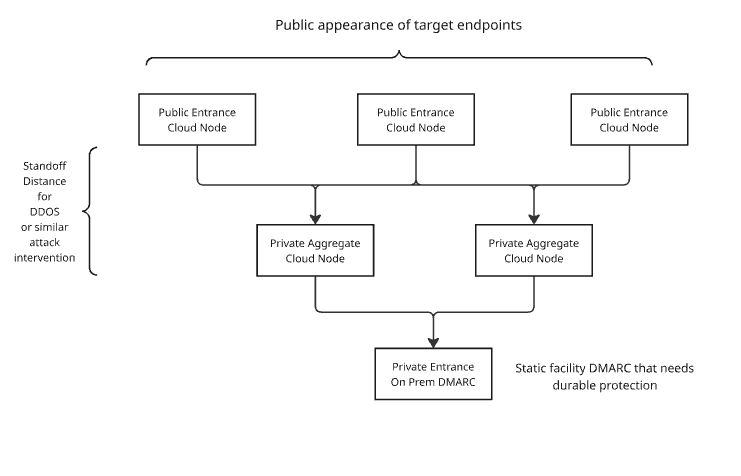
\includegraphics[width=\linewidth]{figures/public to private}}}
  \caption{Your caption}
  \label{fig:your-figure}
\end{figure}

\subsection{Gaps in the Literature}
\section{Methodology}
\subsection{Technical Research Questions}
\subsection{System Architecture and Design}
\subsection{Implementation Plan}
We're starting with a Dell T610 Server.  Made in 2011, this machine is about ten years old.  We purchased this at a government e-waste auction.  She needed some cleanup.  We started on the front lawn, blowing out the dust with a leafblower.

Most of the time servers from these auctions will have minimal \gls{ram}.  Usually the drives and any good accessories will be stripped out.  Anytime we get a hard drive, from any source, one of the first actions we take is to erase the drives to \gls{us} \gls{nist} 800-88 Purge\index{NIST 800-88!Purge}\endnote{Chandramouli, Ramaswamy. Guidelines for Media Sanitization. 2025, \url{nvlpubs.nist.gov/nistpubs/SpecialPublications/nist.SP.800-88r2.pdf}, \url{https://doi.org/10.6028/nist.sp.800-88r2}.} with dedicated devices.  That kind of erasing can be done with \index{dd}\texttt{dd} in Kali or \index{FreeBSD}FreeBSD; but, the drive erasers usually have a verification feature that's helpful.
\subsubsection{Hardware \Gls{configuration}}
This is my favorite computer.  I've named her "Blondie" after Debbie Harry's New Wave band.\endnote{“Blondie | the Official Website of Blondie, Featuring Tour Dates, Presale Ticketing, News, the Official Store and More.” \url{Blondie.net}, 2026, blondie.net/. Accessed 10 June 2026.}

Now, she's configured with:
\begin{itemize}
	\item A \gls{dvd} \gls{rw} drive
    	\item A \index{LTO III tape} \gls{lto} III\endnote{“LTO Ultrium 3: Product Views | Fujifilm [United States].” Fujifilm.com, 2026, \url{www.fujifilm.com/us/en/business/data-storage/data-storage-media/lto-ultrium-3/product-views}. Accessed 10 June 2026.} tape \gls{backup} unit
    	\item In her 8 drive bay, we have:
	\begin{itemize}
		\item Two VelociRaptor\endnote{''WD VelociRaptor ® \GLS{sata} Hard Drives'' \url{https://theretroweb.com/storage/documentation/wd6000-velociraptor-68407cb5c0c96653507203.pdf}} 80GB 10000 rpm drives.
		\begin{itemize}
			\item We'll use these in a \Gls{mirror} \gls{configuration} to hold the main \gls{os}.
		\end{itemize}
		\item Two refurb 120GB \GLS{ssd}s
		\begin{itemize}
			\item We'll use this in a \Gls{mirror} as \gls{zfs} log drives.
			\item They'll help to make writes faster.
		\end{itemize}
		\item Four 500GB hard drives
		\begin{itemize}
			\item We'll use this as a \index{RAIDZ-2}RAIDZ-2 array to hold the \glspl{jail}.
			\item We have some smaller \GLS{sas} drives.
			\item We have some \GLS{sata} drives.
		\end{itemize}
		\end{itemize}
		\item We replaced the one CPU with two Xeon 5550\endnote{Intel® Xeon® Processor 5500 Series an Intelligent Approach to IT Challenges. \url{www.intel.com/content/dam/doc/product-brief/xeon-5500-server-brief.pdf.}} quad cores and added a cooling tower.
		\item We added more \gls{ram}.  Currently, we're at 196GB.
		\item We added some more \gls{nic}s.
		\begin{itemize}
			\item We have four for the jails.
			\item We have two for the \gls{os}.
			\item We'll leave the two on the  \gls{motherboard} mostly unused, except for our iDRAC connection.
			\begin{itemize}
				\item iDRAC is a proprietary baseboard controller.
				\item We could use it to power cycle the machine.
				\item There's a web interface that let's us know about  \gls{motherboard}-related facts.
				\item We cannot give a \index{geli}GELI \gls{password} through the console in our current setup.
			\end{itemize}
	\end{itemize}
	\item The server has two 500W power supplies.
\end{itemize}
Because the dual power supplies draw about 500 Watts apiece, this server gets it own circuit.

The drives we're using are older, but we got enough copies of the drives to be able to support backups.  When making physical backups of the drives, it can be helpful to have other volumes of the same model.  So, instead of getting the best available, we planned for the best we could afford at quantity.

The server does not have:
\begin{itemize}
	\item Any type of graphics card or \gls{gpu}
	\item Sound cards or microphone hardware
	\item Wireless networking or Bluetooth.
\end{itemize}
\subsubsection{Intentions:  Paving the Road to Jails}
We'll use the box for development.  It'll be our main development server.  We'll use it with prog\gls{ram}s that we compile on a nearby \gls{poudriere} package building box.  In those package builds, we have segregated our builds into a pattern of jails that mimic the types of jails that will be needed on most of our computers.

So, there is a \gls{jail} for functional groups like:  development tools, offensive and defensive security programs, browsers, desktop software, and so on.  \gls{poudriere} jails can be filled with whatever sets of programs we like.  For successful builds, we find its best to keep the jails small.

There will be three main groups of drives:
\begin{itemize}
	\item an \gls{os} \Gls{mirror} pair
	\item a \gls{zfs} log \Gls{mirror} pair
	\item a \gls{zfs} \index{RAIDZ-2}RAIDZ-2 kit of four drives.
\end{itemize}

The \gls{os} pair will hold ideas like:
\begin{itemize}
	\item \gls{jail} \gls{configuration}
	\item main host networking and \gls{vnet}
	\item host-based user accounts and \gls{configuration}.
\end{itemize}

The \index{ZFS} \gls{zfs} kits will hold disconnected \index{jails}jails.  We'll set up a system of \index{hierarchical jails}hierarchical jails that provide us with a development environment made up of modular \index{jails}jails that will be the children of an overarching parent.  These \index{jails}jails will communicate with each other and the parent through some custom \gls{vnet}.  We'll do all of our \gls{jail} scripting, controls, and \gls{configuration} manually.  Likewise, the base \index{ZFS} \gls{zfs} setup will be done with simple scripts.
%------------------------------------------------


\subsubsection{Preparing the Baseboard}

The T610 has a built-in  \gls{raid} card that can't be totally bypassed.  This means that since we'll want \index{ZFS} \gls{zfs} to control the drives as much as possible, we'll need to tell the hardware  \gls{raid} to buzz off.  We won't want \index{hardware RAID}hardware  \gls{raid} to participate in the process.  We'll just use the \index{software RAID}software  \gls{raid} through \index{ZFS} \gls{zfs}.

We can't just unplug the  \gls{raid} card.  We tried that, and it leads to malfunctions on this machine.  So, as a compromise, what we'll tell the machine is that each drive is its own \index{VDEV}VDEV and it's \index{RAID-0} \gls{raid}-0.  We'll end up with as many \index{VDEVs}VDEVs as we have physical drives.

To prepare for a later step in this process, we'll note the \index{serial number}serial number of each drive we load into position, its model number, and its capacity.  We'll need to know that information, and we won't want to be hassled by having to power cycle the machine in the middle of the setup process just to check on those details.

Later on, we'll set \index{VDEVs}VDEVs with \index{ZFS} \gls{zfs}; but, from this point on, we'll basically ignore the  \gls{raid} card's description of these devices as VDEVs.

With the baseboard prepared, and the BIOS set to allow us to boot from disc, we'll get started with a plain install of \index{FreeBSD}FreeBSD to the first two drives in a \Gls{mirror} \gls{configuration}.

\subsubsection{Incremental Advancement to \Gls{amnesiac} System}
With all of the manual \index{coding} \gls{coding} and \gls{configuration} needed to set up an \gls{amnesiac} system like the one we desired, it was a big change from the normal \gls{bsd} installs we had done for several years.  Our first pass at building an \gls{amnesiac} system decayed into manually scripting a regular \index{operating system} \gls{operating system} installation that had most of the features we desired in the \gls{amnesiac} system.  Both the on-disc \gls{os} system and the \gls{amnesiac} system are detailed below.

\subsubsection{Identifying and Allocating \gls{zfs} Drive Qualities}
We need to be able to detect the drives and partitions that we want to work with using geom, \index{gpart}gpart, and \gls{zfs} commands.  If, for some reason, you can't find those drives, then you need to address that.  While working with this particular computer, I've found that the leading cause of failing to detect a drive goes back to the VDEV assignment in the hardware  \gls{raid}.  If the drive were pulled, this particular  \gls{raid} card will need to have those \gls{configuration} changes addressed.  Often, this means rebooting the machine.  It could be done through the iDRAC baseboard controller in some models; but the one we have here is not configured to do those tasks.

\subsubsection{What are we going to want the \gls{zfs} kit to do?  How are we going to use the drives?  How can we wrestle with this new type of \gls{configuration}?}
\begin{table}
  \centering
  \caption{\gls{zfs} Concepts and Commands}
  \label{tab:zfsconcepts}
  \begin{tabular}{@{}p{0.30\linewidth} p{0.30\linewidth} p{0.40\linewidth}@{}}
    \toprule
    Topic & Concept & Command phrase example \\
    \midrule
    Disk labels & Use the label to associate the logical with the physical\endnote{Lucas, Michael W, and Allan Jude. FreeBSD Mastery: \gls{zfs}. Tilted Windmill Press, 21 May 2015.} &
      \texttt{[Host]-[PositionNumber 0-7]-[Serial\_Number]}\endnote{This pattern of coordinating host computer, bay position, and drive serial number was recommended by Lucas and Jude.  Lucas, Michael W, and Allan Jude. FreeBSD Mastery: \gls{zfs}. Tilted Windmill Press, 21 May 2015.}\\
    \gls{zfs} Compression & Faster performance: less space\endnote{Lucas, Michael W, and Allan Jude. FreeBSD Mastery: \gls{zfs}. Tilted Windmill Press, 21 May 2015.} &
      \texttt{zfs\index{zfs} set compress=gzip-6 [DIRECTORY]}\endnote{zfs set shown in:  “Zfs\index{zfs}.” Freebsd.org, 2025, \url{man.freebsd.org/cgi/man.cgi?query=zfs&apropos=0&sektion=0&manpath=FreeBSD+14.0-RELEASE&arch=default&format=html}. Accessed 10 June 2026.}  \\
    \gls{zfs} \index{zpool!comment}zpool comment& Make a note on the pool\endnote{Lucas, Michael W, and Allan Jude. FreeBSD Mastery: \gls{zfs}. Tilted Windmill Press, 21 May 2015.} &
      \texttt{zfs set comment="-"}\endnote{\gls{zfs} set shown in:  “Zfs.” Freebsd.org, 2025, \url{man.freebsd.org/cgi/man.cgi?query=zfs&apropos=0&sektion=0&manpath=FreeBSD+14.0-RELEASE&arch=default&format=html}. Accessed 10 June 2026.}  \\
    quota\endnote{“Chapter 6 Managing \gls{zfs} File Systems (Solaris \gls{zfs} Administration Guide).” \url{Docs.oracle.com, docs.oracle.com/cd/E19120-01/open.solaris/817-2271/6mhupg6m3/index.html}.}& Limit growth\endnote{Lucas, Michael W, and Allan Jude. FreeBSD Mastery: \gls{zfs}. Tilted Windmill Press, 21 May 2015.} & --- \\
    reservation\endnote{“Chapter 6 Managing \gls{zfs} File Systems (Solaris \gls{zfs} Administration Guide).” \url{Docs.oracle.com, docs.oracle.com/cd/E19120-01/open.solaris/817-2271/6mhupg6m3/index.html}.} & Set aside space for directory and its children\endnote{Lucas, Michael W, and Allan Jude. FreeBSD Mastery: \gls{zfs}. Tilted Windmill Press, 21 May 2015.} & --- \\
    refreservation\endnote{“Chapter 6 Managing \gls{zfs} File Systems (Solaris \gls{zfs} Administration Guide).” \url{Docs.oracle.com, docs.oracle.com/cd/E19120-01/open.solaris/817-2271/6mhupg6m3/index.html}.} & Set aside space but don't count snapshots and child datasets\endnote{Lucas, Michael W, and Allan Jude. FreeBSD Mastery: \gls{zfs}. Tilted Windmill Press, 21 May 2015.} & --- \\
    canmount\endnote{“Chapter 6 Managing \gls{zfs} File Systems (Solaris \gls{zfs} Administration Guide).” \url{Docs.oracle.com, docs.oracle.com/cd/E19120-01/open.solaris/817-2271/6mhupg6m3/index.html}.}& Control mounting\endnote{Lucas, Michael W, and Allan Jude. FreeBSD Mastery: \gls{zfs}. Tilted Windmill Press, 21 May 2015.} & \texttt{zfs\index{zfs} set canmount=off [DIRECTORY]}\endnote{zfs\index{zfs} set shown in:  “Zfs.” Freebsd.org, 2025, \url{man.freebsd.org/cgi/man.cgi?query=zfs&apropos=0&sektion=0&manpath=FreeBSD+14.0-RELEASE&arch=default&format=html}. Accessed 10 June 2026.}  \\
    mountpoint\endnote{“Chapter 6 Managing \gls{zfs} File Systems (Solaris \gls{zfs} Administration Guide).” \url{Docs.oracle.com, docs.oracle.com/cd/E19120-01/open.solaris/817-2271/6mhupg6m3/index.html}.}& Specify where to mount\endnote{Lucas, Michael W, and Allan Jude. FreeBSD Mastery: \gls{zfs}. Tilted Windmill Press, 21 May 2015.} & \texttt{zfs set mountpoint=/SOME [DIRECTORY]}\endnote{zfs set shown in:  “Zfs\index{zfs}.” Freebsd.org, 2025, \url{man.freebsd.org/cgi/man.cgi?query=zfs&apropos=0&sektion=0&manpath=FreeBSD+14.0-RELEASE&arch=default&format=html}. Accessed 10 June 2026.}  \\
    readonly\endnote{“Chapter 6 Managing \gls{zfs} File Systems (Solaris \gls{zfs} Administration Guide).” \url{Docs.oracle.com, docs.oracle.com/cd/E19120-01/open.solaris/817-2271/6mhupg6m3/index.html}.} & Control readonly\endnote{Lucas, Michael W, and Allan Jude. FreeBSD Mastery: \gls{zfs}. Tilted Windmill Press, 21 May 2015.} & \texttt{zfs set readonly=off [DIRECTORY]}\endnote{\gls{zfs} set shown in:  “Zfs\index{zfs}.” Freebsd.org, 2025, \url{man.freebsd.org/cgi/man.cgi?query=zfs&apropos=0&sektion=0&manpath=FreeBSD+14.0-RELEASE&arch=default&format=html}. Accessed 10 June 2026.}  \\
    exec\endnote{“Chapter 6 Managing \gls{zfs} File Systems (Solaris \gls{zfs} Administration Guide).” \url{Docs.oracle.com, docs.oracle.com/cd/E19120-01/open.solaris/817-2271/6mhupg6m3/index.html}.} & Control if it can execute\endnote{Lucas, Michael W, and Allan Jude. FreeBSD Mastery: \gls{zfs}. Tilted Windmill Press, 21 May 2015.} & \texttt{zfs\index{zfs} set exec=off [DIRECTORY]}\endnote{zfs set shown in:  “Zfs.” Freebsd.org, 2025, \url{man.freebsd.org/cgi/man.cgi?query=zfs&apropos=0&sektion=0&manpath=FreeBSD+14.0-RELEASE&arch=default&format=html}. Accessed 10 June 2026.}  \\
    copies\endnote{“Chapter 6 Managing \gls{zfs} File Systems (Solaris \gls{zfs} Administration Guide).” \url{Docs.oracle.com, docs.oracle.com/cd/E19120-01/open.solaris/817-2271/6mhupg6m3/index.html}.} & Make more than one copy\endnote{Lucas, Michael W, and Allan Jude. FreeBSD Mastery: \gls{zfs}. Tilted Windmill Press, 21 May 2015.} & \texttt{zfs set copies=2 [DIRECTORY]}\endnote{zfs set shown in:  “Zfs\index{zfs}.” Freebsd.org, 2025, \url{man.freebsd.org/cgi/man.cgi?query=zfs&apropos=0&sektion=0&manpath=FreeBSD+14.0-RELEASE&arch=default&format=html}. Accessed 10 June 2026.}  \\
    \bottomrule
  \end{tabular}
\end{table}

After reading over \index{FreeBSD Mastery:  ZFS}FreeBSD Mastery:  \gls{zfs} by Alan Jude and Michael Lucas\endnote{Lucas, Michael W, and Allan Jude. FreeBSD Mastery: \gls{zfs}. Tilted Windmill Press, 21 May 2015.}, we came to a few conclusions.  We chose to use \index{RAIDZ-2}RAIDZ-2 with Log drives because of the number of drives we have\endnote{Lucas and Jude provide a detailed breakdown of different  \gls{raid} and \gls{raid}-Z combinations with differing numbers of drives.  Their analysis and provided charts were our cheif reason for settling in on RAIDZ2.  Lucas, Michael W, and Allan Jude. FreeBSD Mastery: \gls{zfs}. Tilted Windmill Press, 21 May 2015.}.  Some of the topics covered in that book that we'll want to apply include ideas in Table \ref{tab:zfsconcepts}.  In our first iterations we decided to install the \gls{os} on the hard drives in a pattern that looks like a conventional installation.  Once the drive partitioning and utilitization commands were worked out, we then started over and undertook the \index{amensiac} \gls{amnesiac} version with the \gls{os} on a live disc that runs with attached drives.


Our goal for the system will be to split up the drives into three main groups, as described in Tables \ref{tab:zfsmainuseosharddisk}, \ref{tab:zfsjailuseosharddisk}, and \ref{tab:zfsslogusedisk}.  On each drive, we'll also allow:
\begin{itemize}
	\item 15\% of the disk's own capacity as "Free Space" by allocating a blank \gls{partition}
	\item Swap by 100 | 50 | 33 | 25 percent of \gls{ram} (with a 25\% minimum for all disks) or similar
	\item Remainder as one large \gls{zfs} main \gls{partition}.
\end{itemize}
We decided we would want those qualities in an \index{amensiac} \gls{amnesiac} system, with the exception of running the \gls{os} from a live disc.

For the \gls{os}-On-Disk system, this should bring us:
\begin{itemize}
\item Enough room for the main \gls{os}
\item A 4 disk \index{RAIDZ-2}RAIDZ-2 array of almost 1.49 TB of actual storage
\item Fast swap and copy-on-write
\item With each disk capable of expansion or change.
\end{itemize}
The unused space on the drives (a blank \gls{partition} of 15\%) may look like we're grossly under-utilizing the disks.  We're planning for future emergencies.  Do we need more swap?  Maybe we can add it in.  Do we need to expand or resize the disk?  Maybe we can delete that blank "Free Space" partition\index{partition} and use that.  By not trying to use everything, we're giving ourselves some room to solve future problems.

\begin{table}
  \centering
  \caption{\gls{zfs} Main OS Use Hard Disk: Initial Estimates}
  \label{tab:zfsmainuseosharddisk}
  \begin{tabular}{@{}p{0.60\linewidth} p{0.35\linewidth}@{}}
    \toprule
    & Estimate for 80\,\gls{gb} HDD \\
    \midrule
    Blank: 15\% "Free Space" & 12\,GB \\
    Swap: Under-allocate, deliberately & 10\,\gls{gb} \\
    \gls{zfs} Main \gls{partition}: Remainder & 58\,\gls{gb} \\
    \bottomrule
  \end{tabular}
\end{table}

\begin{table} \centering \caption{\gls{zfs} \gls{jail} Use Hard Disk: Initial Estimates} \label{tab:zfsjailuseosharddisk} \begin{tabular}{@{}p{0.60\linewidth} p{0.35\linewidth}@{}} \toprule & Estimate for 500\,\gls{gb} HDD \\ \midrule Blank: 15\% "Free Space" & 75\,GB \\ Swap: 25\% Physical \gls{ram} (196\,GB max) & 50\,GB \\ ZFS Main Partition: Remainder & 375\,GB \\ \bottomrule \end{tabular} \end{table}


\begin{table} \centering \caption{\gls{zfs} SLOG Log Use \GLS{ssd}: Initial Estimates} \label{tab:zfsslogusedisk} \begin{tabular}{@{}p{0.60\linewidth} p{0.35\linewidth}@{}} \toprule & Estimate for 120\,\gls{gb} \GLS{ssd} \\ \midrule Blank: 15\% "Free Space" & 18\,GB \\ Swap: 25\% Physical \gls{ram} (196\,GB max) & 50\,GB \\ ZFS Log Partition: Remainder & 52\,GB \\ \bottomrule \end{tabular} \end{table}


\subsubsection{What We Can Learn From Installing an \gls{os}}
Later on, we'll install the other drives wtih \index{gpart}gpart and \gls{zfs} commands.  This first pair, through, we could do with \index{bsdinstall}bsdinstall\endnote{ “bsdinstall.'' Freebsd.org, 2025, \url{man.freebsd.org/cgi/man.cgi?query=bsdinstall&apropos=0&sektion=0&manpath=FreeBSD+10.3-RELEASE&arch=default&format=html}. Accessed 10 June 2026.}.  If we choose that, though, then we must commit the whole disk to the process.  That would be how we would normally stand up a disk drive.  In this case, we'll conduct a manual process that mimics the main steps of \index{bsdinstall}bsdinstall\endnote{Ibidem.} to show that the installation can be done manually.  Part of these same kinds of steps are critical tasks when administrating and installing jails.

\subsubsection{Basic \index{operating system} \Gls{operating system} Installation Goals}
We're going to do an early phase, basic installation of the \gls{os}.  At this point, we'll really only set up a pair of users and some plain vanilla settings for the \gls{os}.  We want to be able to:
\begin{itemize}
\item to establish our \gls{zfs} kit
\item to configure our main \gls{jail} relationships
\item to be able to check our networking with other hosts
\item to set the basic \index{operating system} \gls{operating system} to call packages from our package server.
\end{itemize}
We can come back later and make a more sophisticated environment.  At this stage, we will just lay the foundation for that work.  If we don't get the \gls{zfs} kit stood up, then our more complex work with jails won't have an environment in which to thrive.


\subsubsection{Main Steps for FreeBSD Installation from \index{bsdinstall}bsdinstall}
\protect\endnote{"bsdinstall.'' Freebsd.org, 2025, \url{man.freebsd.org/cgi/man.cgi?query=bsdinstall&apropos=0&sektion=0&manpath=FreeBSD+10.3-RELEASE&arch=default&format=html}}

We can see that \index{bsdinstall}\texttt{bsdinstall}\endnote{"bsdinstall.'' Freebsd.org, 2025, \url{man.freebsd.org/cgi/man.cgi?query=bsdinstall&apropos=0&sektion=0&manpath=FreeBSD+10.3-RELEASE&arch=default&format=html}} is broken up into about a dozen main segments.  They are:
\begin{itemize}
\item Keyboard mapping
\item Hostname
\item Networking \gls{configuration}
\item Wireless networking
\item Partitioning
\item Mounting temporary root
\item Fetch the \gls{os}
\item Extract the \gls{os}
\item Set a root \gls{password}
\item Set the time
\item Add users
\item Enable some services
\item Copy in the config [2].
\end{itemize}

We're not going to do all of these.  We'll start with partitioning.  We won't do any wireless networking or set a root \gls{password}.  We're going to skip the wireless networking for now because the hardware doesn't have that capability.  In the newer versions of bsdinstall, there are some protective measures not listed above.  We won't tackle those just yet.

\subsubsection{No Root \gls{password}}

We won't set a root \gls{password} because we will expect to always \gls{ssh} into the root account with a key.  By not setting a root \gls{password}, we will create a situation where a key is always required.  This can be dangerous in that it can create a single point of failure for the system.

Another risk is that we will require the ability to \gls{ssh} in as root.  Later, as we establish software firewalls on the host, we will want to limit what addresses can be used to access this root with \gls{ssh}.  It's a little dangerous, but it's also a little different.

We have some risk controls that will be in place.  First, we often store our keys in a special collection of \index{USB!drive}USB drives.  Next, we will have \index{2FA}2FA on the \gls{ssh} that will require a \index{TOTP}TOTP (Time-based One Time \gls{password}).  Finally, we will limit what's done in this drive.  Since most of our programs and work will be done in the jails, there is a limited amount of influence that this part of the system will have.  It's there to start the box and spin up the \index{jails}jails.  If we ever have to totally destroy this installation and hook up our \index{jails}jails to another system, that is possible.

What do we gain from no root \gls{password}?  An extra measure of security.  If there is no \gls{password}, then \gls{password} enumeration attempts should all fail.  This not only goes for root, but it goes for other users.  Many of the automated login attacks we've seen have been simple dictionary attacks; these brute force exercises rarely attempt to account for the types of login procedures that we expect to put in place.

Not having a root \gls{password} may also truncate or stop our ability to use commands like \texttt{\index{su}su} or \texttt{\index{sudo}sudo}.  As we're trying to stop privilege escalation, we'll also be stopping legitimate means of priv-esc.  It could be inconvenient, but we've used this technique before.

Also, there is another risk:  leaving the needed key lying around.  For example, if we give the key to a user account operator, like ourselves, and then we import copies of the key to the box for easy use:  well, then those keys could be used and re-used locally.  This would be the equivalent for storing a plain-text \gls{password} on the box.  They keys are ultimately simple text files with decorated, long, strings of hashes.  It's the software that goes with the keys, combined with the \gls{configuration} of the prog\gls{ram}s for logging in to a service, that makes them special.  Switching from passwords to keys is not a perfect answer; but, it's the answer we'll use this time.

If someone wishes to put a root \gls{password} in place, then that's a procedure that will be easy to implement.  For now, though, there will be no root \gls{password}.  And that means we have to build the keys we will use to log in.

\subsubsection{Be Able to Build the Keys}
We can build our keys using the live disc's  \gls{shell}. and a  \gls{thumbdrive}.  The main command to build the keys is:\\\\
\texttt{\index{ssh-keygen}ssh-keygen -b 1024 -t rsa}\endnote{“ssh-Keygen.” Freebsd.org, 2025, \url{man.freebsd.org/cgi/man.cgi?query=ssh-keygen&apropos=0&sektion=0&manpath=FreeBSD+10.3-RELEASE&arch=default&format=html}. Accessed 10 June 2026.}\\

Copy the files output to a  \gls{thumbdrive} and keep them handy for mounting.

\subsubsection{\gls{partition}, Mount, and Use a  \Gls{thumbdrive} from Live Disc's  \Gls{shell}}
Let's take some time to go over some detailed instructions on how to build those keys and get them onto a  \gls{thumbdrive}.  The live disc's  \gls{shell} mostly uses a read-only file system.  So, some people may not be familiar with how we are going to get the keys made and saved anywhere that will persist.
\subsubsection{Start the Box and the Live Disk's  \Gls{shell}}
With the hardware booted to the LiveCD (installation disc), we select " \Gls{shell}" from the three main choices in the first menu.  This drops us into the  \gls{shell}.  If we try to save a file of any kind, we'll probably get an error message back that says we're in a read-only file system.
Our main set of directions for this is in the \index{FreeBSD Handbook}FreeBSD Handbook.  We look carefully at the sections for USB storage and "Adding Disks"
\subsubsection{Be Able to Plug in the USB  \Gls{thumbdrive} and Find Its Logical Address}

\texttt{\index{camcontrol!devlist}camcontrol devlist}\endnote{“camcontrol.” Freebsd.org, 2025, \url{man.freebsd.org/cgi/man.cgi?query=camcontrol&apropos=0&sektion=0&manpath=FreeBSD+10.3-RELEASE&arch=default&format=html}. Accessed 10 June 2026.}\\

This should show the USB drive.  If the list is long, we can  \gls{pipe} it to more and slowly advance through the list.  In our case, the USB was at da0.

The listing should also show any other storage device that's plugged in to the machine.  So, all of those hard drives loaded into the bays should appear.  If they don't, then take it as a warning sign that we're having a problem with the  \gls{raid} card's physical drive VDEVs.  On the T610, we were seeing drives in positions 0 to 7 in addition to the USB  \gls{thumbdrive} we're working on now.

\subsubsection{Be Able to \gls{partition} the USB}
Since our USB has not been prepared for use with anything, we have to \gls{partition} it.  We can pretty much use the default commands fro 17.2 "Adding Disks" to set up the drive.  Here, we create a simple UFS file system and mount it to a directory that we'll put in /tmp. If our USB is already partitioned, we would want to skip this part.  \\\\
\texttt{\index{gpart!create}gpart create -s GPT da0}\endnote{“gpart(8).” Freebsd.org, 2026, \url{man.freebsd.org/cgi/man.cgi?query=gpart&apropos=0&sektion=8&manpath=FreeBSD+10.3-RELEASE&arch=default&format=html}. Accessed 10 June 2026}\\
\texttt{\index{gpart!add}gpart add -t freebsd-ufs -a 1M da0}\endnote{Ibidem.}\\
\texttt{\index{newfs}newfs -U /dev/da0p1}\endnote{“newfs.” Freebsd.org, 2025, \url{man.freebsd.org/cgi/man.cgi?query=newfs&apropos=0&sektion=0&manpath=FreeBSD+10.3-RELEASE&arch=default&format=html}. Accessed 10 June 2026.}\\\\
Mount the USB to the /tmp Directory:\\\\
\texttt{\index{mkdir}mkdir /tmp/someDir}\endnote{“Mkdir.” Freebsd.org, 2025, \url{man.freebsd.org/cgi/man.cgi?query=mkdir&apropos=0&sektion=0&manpath=FreeBSD+10.3-RELEASE&arch=default&format=html}. Accessed 10 June 2026.}\\
\texttt{\index{mount}mount /dev/da0p1 /tmp/someDir}\endnote{“Mount.” Freebsd.org, 2025, \url{man.freebsd.org/cgi/man.cgi?query=mount&apropos=0&sektion=0&manpath=FreeBSD+10.3-RELEASE&arch=default&format=html}. Accessed 10 June 2026.}\\

\subsubsection{Be Able to Write to the USB}
We could now write a simple text file onto /tmp/someDir, unmount the drive, and then re-mount it to check our work.  That would go like:\\\\
\texttt{\index{cd}cd /tmp}\endnote{“cd.” Freebsd.org, 2025, \url{man.freebsd.org/cgi/man.cgi?query=cd&apropos=0&sektion=0&manpath=FreeBSD+10.3-RELEASE&arch=default&format=html}. Accessed 10 June 2026.}\\
\texttt{\index{umount}umount /tmp/someDir}\endnote{“umount.” Freebsd.org, 2025, \url{man.freebsd.org/cgi/man.cgi?query=umount&apropos=0&sektion=0&manpath=FreeBSD+10.3-RELEASE&arch=default&format=html}. Accessed 10 June 2026.}\\
\texttt{\index{rm}rm -r /tmp/someDir}\endnote{“rm.” Freebsd.org, 2025, \url{man.freebsd.org/cgi/man.cgi?query=rm&apropos=0&sektion=0&manpath=FreeBSD+10.3-RELEASE&arch=default&format=html}. Accessed 10 June 2026.}\\\\
Unplug the drive.  Plug it in another slot.  Use camcontrol devlist to find it again.  It'll probably get the same address, like "da0".\\\\
\texttt{\index{mkdir}mkdir /tmp/otherDir}\endnote{“Mkdir.” Freebsd.org, 2025, \url{man.freebsd.org/cgi/man.cgi?query=mkdir&apropos=0&sektion=0&manpath=FreeBSD+10.3-RELEASE&arch=default&format=html}. Accessed 10 June 2026.}\\
\texttt{\index{mount}mount /dev/da0p1 /tmp/otherDir}\endnote{“Mount.” Freebsd.org, 2025, \url{man.freebsd.org/cgi/man.cgi?query=mount&apropos=0&sektion=0&manpath=FreeBSD+10.3-RELEASE&arch=default&format=html}. Accessed 10 June 2026.}\\
\texttt{\index{ls}ls /tmp/otherDir}\endnote{“ls.” Freebsd.org, 2025, \url{man.freebsd.org/cgi/man.cgi?query=ls&apropos=0&sektion=0&manpath=FreeBSD+10.3-RELEASE&arch=default&format=html}. Accessed 10 June 2026.}\\

\subsubsection{Be Able to Put Some Key Pairs on the USB}
Using these same principles, we can mount our USB  \gls{thumbdrive}, generate \gls{ssh} keys, and save them there for later.\\\\
\texttt{\index{mkdir} mkdir /tmp/otherDir/keys}\endnote{“Mkdir.” Freebsd.org, 2025, \url{man.freebsd.org/cgi/man.cgi?query=mkdir&apropos=0&sektion=0&manpath=FreeBSD+10.3-RELEASE&arch=default&format=html}. Accessed 10 June 2026.}\\
\texttt{\index{ssh-keygen} ssh-keygen -b 1024 -t rsa}\endnote{“ssh-Keygen.” Freebsd.org, 2025, \url{man.freebsd.org/cgi/man.cgi?query=ssh-keygen&apropos=0&sektion=0&manpath=FreeBSD+10.3-RELEASE&arch=default&format=html}. Accessed 10 June 2026.}\\

During the ssh-keygen  \index{dialog} \gls{dialog}, simply direct the prog\gls{ram} to save the keys to \texttt{/tmp/otherDir/keys}.  Be sure to record your \gls{passphrase} somewhere.

\subsubsection{Be Able to Use Commands to Build Out the Drives}
We'd like to show a quick overview of some of the drive-related commands.  These will be applied soon.

To list what devices are detected by the \gls{os}, we can use:\\\\
\texttt{ \index{gpart}gpart show}\endnote{“gpart(8).” Freebsd.org, 2026, \url{man.freebsd.org/cgi/man.cgi?query=gpart&apropos=0&sektion=8&manpath=FreeBSD+10.3-RELEASE&arch=default&format=html}. Accessed 10 June 2026.}\\\\
We will want to note the serial number of each drive, by position.
We then note which drives we want to use for the main body of the \index{RAIDZ-2}RAIDZ-2 kit.  All of this will become one pool of \gls{zfs} VDEVs.  Then we'll add in the log \gls{mirror}s.  So, in the sequence of 0-7, numbering the drives, we should expect to skip those two for now.

Make the notes if you haven't already because we're going to list all of the drives for the main pool in one pop.  This task may have been done before we set up the physical VDEVs for the hardware  \gls{raid}.

We're going to choose to put a swap \gls{partition} on the \GLS{ssd}s.  We can add one onto the other disks, but a maximum of 4 swap partitions is recommended in the \index{FreeBSD Handbook}FreeBSD Handbook.  Later on, we will be able to select swap partitions by mounting them and using commands like \texttt{\index{swapon}swapon swapoff}.\\

To put the \gls{zfs} \gls{partition} on the remaining disks:\\\\
\texttt{ \index{gpart!create}gpart create -s SCHEME DISK\_DEVICE}\endnote{“gpart(8).” Freebsd.org, 2026, \url{man.freebsd.org/cgi/man.cgi?query=gpart&apropos=0&sektion=8&manpath=FreeBSD+10.3-RELEASE&arch=default&format=html}. Accessed 10 June 2026.}\\\\
\texttt{ \index{gpart!create}gpart create -s gpt da4}\endnote{Ibidem.}
\\

To add the main \gls{zfs} \gls{partition}:\\\\
\texttt{ \index{gpart!add}gpart add -a 1m -l \gls{zfs}\_NUMBER \textbackslash\\ -t freebsd-zfs DISK\_DEVICE}\endnote{Ibidem.}\\\\
\texttt{ \index{gpart!add}gpart add -a 1m -l \gls{zfs}-BLONDIE-4-WD123465789 \textbackslash\\-t freebsd-zfs  da4}\endnote{Ibidem.}
\\

To add the \gls{partition}'s swap:\\\\
\texttt{ \index{gpart!add}gpart add -a 1m -slg -l SWAP\_NUMBER \textbackslash\\-t freebsd-swap DISK\_DEVICE}\endnote{Ibidem.}\\\\
\texttt{ \index{gpart!add}gpart add -a 1m -slg -l SWAP-BLONDIE-4-WD123465789 \textbackslash\\-t freebsd-swap da4}\endnote{Ibidem.}
\\

To add a logging \gls{partition} on the SLOG \GLS{ssd}s:\\\\
\texttt{ \index{gpart!add}gpart add -a 1m -l ZLOG\_NUMBER  \textbackslash\\-t freebsd-zfs\index{zfs} DISK\_DEVICE}\endnote{Ibidem.}\\\\
\texttt{ \index{gpart!add}gpart add -a 1m -l ZLOG-BLONDIE-2-WD123465789 \textbackslash\\-t freebsd-zfs  da2}\endnote{Ibidem.}\\\\

With each disk partitioned, we can add them to the pool for our RAIDZ-2 kit.\\\\
\texttt{\index{zpool!create}zpool create \gls{raid} \seqsplit{POOL\_NAME} \seqsplit{DISK\_LABEL}/\gls{zfs}\_\seqsplit{\gls{partition}\_LABEL} ...\seqsplit{next} disk/\gls{partition}...}\endnote{"zpool." Freebsd.org, 2025, \url{man.freebsd.org/cgi/man.cgi?query=zpool&apropos=0&sektion=0&manpath=FreeBSD+10.3-RELEASE&arch=default&format=html}. Accessed 10 June 2026.}\\\\

\noindent\texttt{\index{zpool!create}zpool create BLONDIE-MAIN \index{RAIDZ-2}raidz2 \textbackslash }\endnote{Ibidem.}\\
\texttt{BLONDIE-4-WD12345/ZFS-BLONDIE-4-WD12345 \textbackslash }\\
\texttt{BLONDIE-5-WD12345/\gls{zfs}-BLONDIE-5-WD12345 \textbackslash }\\
\texttt{BLONDIE-6-WD12345/ZFS\index{zfs}-BLONDIE-6-WD12345 \textbackslash }\\
\texttt{BLONDIE-7-WD12345/ZFS-BLONDIE-7-WD12345 }\\

We can add on the \gls{mirror}s for logging:\\\\
\texttt{\index{zpool!add}zpool add BLONDIE-MAIN log \gls{mirror} \textbackslash}\endnote{Ibidem.}\\
\texttt{BLONDIE-2-WD12345/ZLOG-BLONDIE-2-WD12345 \textbackslash}\\
\texttt{BLONDIE-3-WD12345/ZLOG-BLONDIE-3-WD12345}\\


Once we get to the point that we have an \index{operating system} \gls{operating system} on disks, and disks ready for use with logs and jails, then we're at the end of this phase of system administration.

\subsubsection{Goals for \Gls{amnesiac} Systems}
We chose at this point to do some experimental installs.  For clarity, notes on those are not presented here.  We did change our goals for the system.  We recognized that we wanted:
\begin{itemize}
\item Use a LiveCD for an immutable \gls{os}
\item  \index{encrypt} \Gls{encrypt} disc partitions instead of the whole disc
\item Ensure we save keys and  \gls{metadata} to promote disc recovery
\item Prepare commands in advance to reduce complexity.
\end{itemize}

From our testing, we recognizes that a Live CD offered the best answer for an \gls{immutable system}.  It does come at the price of some instability.  The "El Torrito" discs have a limited set of services.  Adjusting the \gls{configuration} of the \index{operating system} \gls{operating system} means drafting, burning, and testing a new disc.  The " \gls{shell}" instance on a \index{FreeBSD}FreeBSD installation disc is reportedly less stable; but, we did not know why or how it was less stable than a normal \index{operating system} \gls{operating system}.  We worked through our disc commands and kept careful notes.  Adding the physical serial number of the disc alone increased the complexity of manually typing in each command.  We discovered the need to  \index{encrypt} \gls{encrypt} the discs by partitions instead of the whole disc because there was a visibility problem during the execution of discovering and attaching the discs.  There was a poorly documented detail about protecting the disc  \gls{metadata} and keys.  The keys are provided during the setup  \index{dialog} \gls{dialog}; but, these highly important items will disappear after the setup process closes.  This means it is important that an operator recognize the need to intercept and to record these keys.  Without them, a later recovery of a disc is impossible.  Since one typo would derail our experimental setups, we had to keep a second support computer on hand to record notes and consult references.

%------------------------------------------------

As our experimentation concluded, we had learned enough to stand a reasonable chance to setup an \gls{amnesiac} machine.  Its features include:

\begin{itemize}
\item An immutable \gls{os}
\item  \index{encrypt} \Gls{encrypt}ed disc partitions
\item Swap and logging for \gls{zfs} disc features
\item  \Gls{metadata} and keys saved to a separate USB drive
\item A disc for holding FreeBSD jails (containerization)
\item Enough room to expand, to update, and to recover.
\end{itemize}

\subsubsection{Configure for SWAP Disk, \gls{zfs}  \index{cache} \Gls{cache}, \gls{zfs} SLOG \Gls{mirror}, and \gls{zfs} RAIDz2}

\begin{table} \centering \caption{FreeBSD Swap Disk — Estimate of 500\,\gls{gb} HDD} \label{tab:freebsdswapdisc} \begin{tabular}{@{}p{0.60\linewidth} p{0.35\linewidth}@{}} \toprule GEOM Disk List Mediasize & 465\,\gls{gb} \\ \midrule Blank: 15\% "Free Space" & 70\,GB \\ Swap & 395\,GB \\ \bottomrule \end{tabular} \end{table}

\begin{table} \centering \caption{\gls{zfs}  \index{cache} \Gls{cache} (Read  \index{cache} \Gls{cache}) Disk — Estimate of 80\,\gls{gb} HDD} \label{tab:zfscachedisc} \begin{tabular}{@{}p{0.60\linewidth} p{0.35\linewidth}@{}} \toprule GEOM Disk List Mediasize & 74\,\gls{gb} \\ \midrule Blank: 15\% "Free Space" & 11\,GB \\ Swap & 63\,GB \\ \bottomrule \end{tabular} \end{table}
\begin{table} \centering \caption{\gls{zfs} SLOG Log \gls{mirror} (Write  \index{cache} \Gls{cache}) Disk — Initial Estimates} \label{tab:zfsslogmirror} \begin{tabular}{@{}p{0.60\linewidth} p{0.35\linewidth}@{}} \toprule & Estimate for 120\,\gls{gb} \GLS{ssd} \\ \midrule GEOM Disk List Mediasize & 465\,\gls{gb} \\ Blank: 15\% "Free Space" & 18\,GB \\ Swap: 25\% Physical \gls{ram} (196\,GB max) & 50\,GB \\ ZFS Log Partition: Remainder & 52\,GB \\ \bottomrule \end{tabular} \end{table}
\begin{table} \centering \caption{\gls{zfs} \gls{jail} Use Hard Disk — Estimate of 500\,\gls{gb} HDD} \label{tab:zfsjailusehdd} \begin{tabular}{@{}p{0.60\linewidth} p{0.35\linewidth}@{}} \toprule & Estimate for 500\,\gls{gb} HDD \\ \midrule GEOM Disk List Mediasize & 465\,\gls{gb} \\ Blank: 15\% "Free Space" & 75\,GB \\ Swap: 25\% Physical \gls{ram} (196\,GB max) & 50\,GB \\ ZFS Main Partition: Remainder & 375\,GB \\ \bottomrule \end{tabular} \end{table}

Changed config to keep the RAIDZ2 for main work.  I was having trouble with the \GLS{ssd}s; so, I removed them and replaced them with two 80GB Western Digital Velociraptors.  I added another WD Velociraptor for  \index{cache} \gls{cache}.  Then we added a Western Digital Blue 500GB for a swap disk.  That sounds like a lot of swap, but we hope to upgrade to near 196GB of \gls{ram} this year. So, a little more than twice that would be 400GB of swap.  The next disk size on hand was 500GB.

We had some mis-aligned partitions with RAIDZ2 work for Blondie.  We were using the full 500GB on the label as our actual amount of media to work with.  Since less is available, we will have to set those up again.

We used  \index{gpart}gpart delete to delete each \gls{partition}.  Then we used  \index{gpart}gpart destroy to delete the \gls{partition} table for the whole disk.  In the end,  \index{gpart}gpart showed us only the CD.

\subsubsection{Startup with \texttt{bootonly.iso}}
For this run, we’ll begin by using the boot-only disk.  We won’t plan to ever boot from these hard drives.  We’ll just use the  \gls{shell} on the CD.  As with the others, we’ll mount a USB to store  \gls{metadata} information.  We’ll \gls{partition} and  \index{encrypt} \gls{encrypt} the disks.  In the following examples, we provide the actual serial numbers for the hard drives that were used.  This example was derived from notes we maintained during experimentation; serial numbers in other instances will vary, of course.

\subsubsection{Mount the USB to Save the  \Gls{metadata} \gls{backup} File}
\texttt{\index{mkdir}mkdir /tmp/usb3}\endnote{“Mkdir.” Freebsd.org, 2025, \url{man.freebsd.org/cgi/man.cgi?query=mkdir&apropos=0&sektion=0&manpath=FreeBSD+10.3-RELEASE&arch=default&format=html}. Accessed 10 June 2026.}\\
\texttt{\index{mount}mount /dev/da0p1 /tmp/usb3}\endnote{“mount.” Freebsd.org, 2025, \url{man.freebsd.org/cgi/man.cgi?query=mount&apropos=0&sektion=0&manpath=FreeBSD+10.3-RELEASE&arch=default&format=html}. Accessed 10 June 2026.}

\subsubsection{Create Swap Disk in Bay 0}
\texttt{\index{gpart!create}gpart create -s GPT mfid0}\endnote{“gpart(8).” Freebsd.org, 2026, \url{man.freebsd.org/cgi/man.cgi?query=gpart&apropos=0&sektion=8&manpath=FreeBSD+10.3-RELEASE&arch=default&format=html}. Accessed 10 June 2026.}\\\
\texttt{\index{gpart!add}gpart add -a 5K -s 395G -t freebsd-swap \textbackslash\\-l \gls{zfs}-BLONDIE-0-SWAP-WCC2ERZ56512 mfid0}\endnote{Ibidem.}

\subsubsection{Create \gls{zfs} \gls{cache} in Bay 1}
\texttt{\index{gpart!create}gpart create -s GPT mfid1}\endnote{Ibidem.}\\\\
\texttt{\index{gpart!add}gpart add -a 5K -s 63G -t freebsd-zfs\index{zfs} \textbackslash\\-l \gls{zfs}-BLONDIE-1-\gls{cache}-WXL1E40C1352 mfid1}\endnote{Ibidem.}

\subsubsection{Create \gls{zfs} SLOG in Bays 2 and 3}
\texttt{\index{gpart!create}gpart create -s GPT mfid2}\endnote{Ibidem.}\\\\
\texttt{\index{gpart!add}gpart add -a 5K -s 63G -t freebsd-zfs \textbackslash\\-l \gls{zfs}-BLONDIE-2-SLOG-WXL1E4067503 mfid2}\endnote{Ibidem.}\\\\
\texttt{\index{gpart!create}gpart create -s GPT mfid3}\endnote{Ibidem.}\\\\
\texttt{\index{gpart!add}gpart add -a 5K -s 63G -t freebsd-zfs \textbackslash\\ -l \gls{zfs}-BLONDIE-3-SLOG-WXC0CA9V8431 mfid3}\endnote{Ibidem.}\\\\

\subsubsection{Create \gls{zfs} Work Disks for Jails}
\subsubsection{Bay 4}
\texttt{\index{gpart!create}gpart create -s GPT mfid4}\endnote{Ibidem.}\\\\
\texttt{\index{gpart!add}gpart add -a 5K -s 50G -t freebsd-swap \textbackslash\\-l \gls{zfs}-BLONDIE-4-SWAP-WCC2EE134983 mfid4}\endnote{Ibidem.}\\\\
\texttt{\index{gpart!add}gpart add -s 345G -t freebsd-\gls{zfs} \textbackslash\\-l \gls{zfs}-BLONDIE-4-FILES-WCC2EE134983 mfid4}\endnote{Ibidem.}
\subsubsection{Bay 5}
\texttt{\index{gpart!create}gpart create -s GPT mfid5}\endnote{Ibidem.}\\\\
\texttt{\index{gpart!add}gpart add -a 5K -s 50G -t freebsd-swap \textbackslash\\-l \gls{zfs}-BLONDIE-5-SWAP-WMC2E3914420 mfid5}\endnote{Ibidem.}\\\\
\texttt{\index{gpart!add}gpart add -s 345G -t freebsd-zfs \textbackslash\\-l \gls{zfs}-BLONDIE-5-FILES-WMC2E3914420 mfid5}\endnote{Ibidem.}
\subsubsection{Bay 6}
\texttt{\index{gpart!create}gpart create -s GPT mfid6}\endnote{Ibidem.}\\\\
\texttt{\index{gpart!add}gpart add -a 5K -s 50G -t freebsd-swap \textbackslash\\ -l \gls{zfs}-BLONDIE-6-SWAP-WCC2ETT39577 mfid6}\endnote{Ibidem.}\\\\
\texttt{\index{gpart!add}gpart add -s 345G -t freebsd-zfs \textbackslash\\-l \gls{zfs}-BLONDIE-6-FILES-WCC2ETT39577 mfid6}\endnote{Ibidem.}
\subsubsection{Bay 7}
\texttt{\index{gpart!create}gpart create -s GPT mfid7}\endnote{Ibidem.}\\\\
\texttt{\index{gpart!add}gpart add -a 5K -s 50G -t freebsd-swap \textbackslash\\-l \gls{zfs}-BLONDIE-7-SWAP-WCAYU2878968 mfid7}\endnote{Ibidem.}\\\\
\texttt{\index{gpart!add}gpart add -s 345G -t freebsd-zfs \textbackslash\\-l \gls{zfs}-BLONDIE-7-FILES-WCAYU2878968 mfid7}\endnote{Ibidem.}\\

We should note that “Bay 7” is an observation of the physical hardware.  The device (“mfid7”) could have whatever number assigned at the end that the machine gave it.  If the hardware  \gls{raid} had a problem with recognizing a device, the number might not correlate to what bay it is in.  When powering up, check your geometry.

\subsubsection{ \index{encrypt} \Gls{encrypt} those partitions}
During this phase, we’ll  \index{encrypt} \gls{encrypt} the partitions.  That means that we should have some recordkeeping materials on hand.  Use a \gls{password} manager or a notebook to carefully record the \gls{password} that is about to be typed in.  With each one completed, the machine will tell us that it has saved a file of \gls{backup}  \gls{metadata}.  We will want to copy that  \gls{metadata} file to the  \gls{thumbdrive}.  If the  \index{encrypt} \gls{encrypt}ion gets jammed up, or if there is some type of problem, then the  \gls{metadata} file will be used as part of the recovery process.  Without a  \gls{metadata} file, recovering an  \index{encrypt} \gls{encrypt}ed \gls{partition} can be difficult or impossible.

If you lose the  \gls{metadata} file, but still have routine access to the \index{geli}geli  \index{encrypt} \gls{encrypt}ion because you know the \gls{password} and the machine is functioning alright, then you can export another copy of the  \gls{metadata}.  This means that anyone with root access to the machine, who can use \index{geli}geli commands, would also be able to export such a file.  Keep this in mind if you need to secure your machine.

When we give the subcommand to “init,” the machine will ask us to give the new \gls{password} twice.  This is part of the \gls{password} setting process.  When we give the subcommand to “attach,” the machine will ask us to give the \gls{password} as part of the normal attachment process. Type carefully, and look at the records carefully, because this is the main chance to make sure the \gls{password} notes are right.

\subsubsection{Commands to  \index{encrypt} \Gls{encrypt} the Partitions}
\texttt{\index{geli!init}geli init -l 256 mfid0p1}\endnote{“Geli(8).” Freebsd.org, 2025, \url{man.freebsd.org/cgi/man.cgi?query=geli&sektion=8&manpath=FreeBSD+10.3-RELEASE}. Accessed 10 June 2026.}\\
\texttt{\index{geli!attach}geli attach mfid0p1}\endnote{Ibidem.}\\\\
\texttt{\index{geli!init}geli init -l 256 mfid1p1}\endnote{Ibidem.}\\
\texttt{\index{geli!attach}geli attach mfid1p1}\endnote{Ibidem.}\\\\
\texttt{\index{geli!init}geli init -l 256 mfid2p1}\endnote{Ibidem.}\\
\texttt{\index{geli!attach}geli attach mfid2p1}\endnote{Ibidem.}\\\\
\texttt{\index{geli!init}geli init -l 256 mfid3p1}\endnote{Ibidem.}\\
\texttt{\index{geli!attach}geli attach mfid3p1}\endnote{Ibidem.}\\\\
\texttt{\index{geli!init}geli init -l 256 mfid4p1}\endnote{Ibidem.}\\
\texttt{\index{geli!attach}geli attach mfid4p1}\endnote{Ibidem.}\\\\
\texttt{\index{geli!init}geli init -l 256 mfid4p2}\endnote{Ibidem.}\\
\texttt{\index{geli!attach}geli attach mfid4p2}\endnote{Ibidem.}\\\\
\texttt{\index{geli!init}geli init -l 256 mfid5p1}\endnote{Ibidem.}\\
\texttt{\index{geli!attach}geli attach mfid5p1}\endnote{Ibidem.}\\\\
\texttt{\index{geli!init}geli init -l 256 mfid5p2}\endnote{Ibidem.}\\
\texttt{\index{geli!attach}geli attach mfid5p2}\endnote{Ibidem.}\\\\
\texttt{\index{geli!init}geli init -l 256 mfid6p1}\endnote{Ibidem.}\\
\texttt{\index{geli!attach}geli attach mfid6p1}\endnote{Ibidem.}\\\\
\texttt{\index{geli!init}geli init -l 256 mfid6p2}\endnote{Ibidem.}\\
\texttt{\index{geli!attach}geli attach mfid6p2}\endnote{Ibidem.}\\\\
\texttt{\index{geli!init}geli init -l 256 mfid7p1}\endnote{Ibidem.}\\
\texttt{\index{geli!attach}geli attach mfid7p1}\endnote{Ibidem.}\\\\
\texttt{\index{geli!init}geli init -l 256 mfid7p2}\endnote{Ibidem.}\\
\texttt{\index{geli!attach}geli attach mfid7p2}\endnote{Ibidem.}\\\\

\subsubsection{To Preserve the  \Gls{metadata} \gls{backup} Files}
Let us reiterate:  preserving these backups at the time of disk creation is essential for later recoveries.  If these files are not saved, then a powerdown of the system will cause them to be lost.  They're automatically stored in an ephemeral directory.  Conserve the ability to recover a disk later by recording these  \gls{metadata} \gls{backup} files to a safe location.

Each  \gls{metadata} \gls{backup} file was probably created with a name that does not look like the drive’s label.  Instead, the machine assigns a \gls{backup} file name based on geometry.  Since we can have a hardware \gls{configuration} change that could mess up that pattern, we will want to save our \gls{backup} files with names that look more like the disk labels.  That way, if the drives move, then we can better discover which  \gls{metadata} file goes with it.\\

\noindent\texttt{\index{cp}cp /var/backups/mfid0p1.eli /tmp/usb3/backups\\\_27SEP2020/\gls{zfs}-BLONDIE-0-SWAP-WCC2ERZ56512.eli}\endnote{“cp.” Freebsd.org, 2025, \url{man.freebsd.org/cgi/man.cgi?query=cp&apropos=0&sektion=0&manpath=FreeBSD+10.3-RELEASE&arch=default&format=html}. Accessed 10 June 2026.}\\\\
\texttt{\index{cp}cp /var/backups/mfid1p1.eli /tmp/usb3/backups\\\_27SEP2020/\gls{zfs}-BLONDIE-1-\gls{cache}-WXL1E40C1352.eli}\endnote{Ibidem.}\\\\
\texttt{\index{cp}cp /var/backups/mfid2p1.eli /tmp/usb3/backups\\\_27SEP2020/\gls{zfs}-BLONDIE-2-SLOG-WXL1E4067503.eli}\endnote{Ibidem.}\\\\
\texttt{\index{cp}cp /var/backups/mfid3p1.eli /tmp/usb3/backups\\\_27SEP2020/\gls{zfs}-BLONDIE-3-SLOG-WXC0CA9V8431.eli}\endnote{Ibidem.}\\\\
\texttt{\index{cp}cp /var/backups/mfid4p1.eli /tmp/usb3/backups\\\_27SEP2020/\gls{zfs}-BLONDIE-4-SWAP-WCC2EE134983.eli}\endnote{Ibidem.}\\\\
\texttt{\index{cp}cp /var/backups/mfid4p2.eli /tmp/usb3/backups\\\_27SEP2020/\gls{zfs}-BLONDIE-4-FILES-WCC2EE134983.eli}\endnote{Ibidem.}\\\\
\texttt{\index{cp}cp /var/backups/mfid5p1.eli /tmp/usb3/backups\\\_27SEP2020/\gls{zfs}-BLONDIE-5-SWAP-WMC2E3914420.eli}\endnote{Ibidem.}\\\\
\texttt{\index{cp}cp /var/backups/mfid5p2.eli /tmp/usb3/backups\\\_27SEP2020/\gls{zfs}-BLONDIE-5-FILES-WMC2E3914420.eli}\endnote{Ibidem.}\\\\
\texttt{\index{cp}cp /var/backups/mfid6p1.eli /tmp/usb3/backups\\\_27SEP2020/\gls{zfs}-BLONDIE-6-SWAP-WCC2ETT39577.eli}\endnote{Ibidem.}\\\\
\texttt{\index{cp}cp /var/backups/mfid6p2.eli /tmp/usb3/backups\\\_27SEP2020/\gls{zfs}-BLONDIE-6-FILES-WCC2ETT39577.eli}\endnote{Ibidem.}\\\\
\texttt{\index{cp}cp /var/backups/mfid7p1.eli /tmp/usb3/backups\\\_27SEP2020/\gls{zfs}-BLONDIE-7-SWAP-WCAYU2878968.eli}\endnote{Ibidem.}\\\\
\texttt{\index{cp}cp /var/backups/mfid7p2.eli /tmp/usb3/backups\\\_27SEP2020/\gls{zfs}-BLONDIE-7-FILES-WCAYU2878968.eli}\endnote{Ibidem.}

\subsubsection{File Name Check:  Editing Labels}
We got through all that, and found that we had named a file incorrectly.  During experimentation, we had a typo; BAY 4 should be
\texttt{WCC2EE134983} but that's not what we saw when we checked our work.  Not the end of the world.  We can move the .eli  \gls{metadata} file, and we can use  \index{gpart!modify}gpart\endnote{“gpart(8).” Freebsd.org, 2026, \url{man.freebsd.org/cgi/man.cgi?query=gpart&apropos=0&sektion=8&manpath=FreeBSD+10.3-RELEASE&arch=default&format=html}. Accessed 10 June 2026.} modify to change the label.\\

\noindent\texttt{ \index{gpart!modify}gpart modify -i 1 \textbackslash\\-l \gls{zfs}-BLONDIE-4-SWAP-WCC2EE134983 mfid4}\endnote{Ibidem.}\\\\
\texttt{ \index{gpart!modify}gpart modify -i 2 \textbackslash\\-l \gls{zfs}-BLONDIE-4-FILES-WCC2EE134983 mfid4}\endnote{Ibidem.}\\

\texttt{ \index{gpart!show}gpart show}\endnote{Ibidem.} and \texttt{\index{geli!status}geli status}\endnote{“geli(8).” Freebsd.org, 2025, \url{man.freebsd.org/cgi/man.cgi?query=geli&sektion=8&manpath=FreeBSD+10.3-RELEASE}. Accessed 10 June 2026.} should show our drives as we expect them to be.

At this point, all of the drives should be partitioned and decrypted and attached.  We can build a \index{zpool}zpool for our \gls{zfs} file system. We can attach that swap drive for the benefit of our \index{operating system} \gls{operating system} right now.

\subsubsection{To Use the Swap Disk}
\noindent\texttt{\index{swapon}swapon mfid0p1.eli}\endnote{“swapon.” Freebsd.org, 2025, \url{man.freebsd.org/cgi/man.cgi?query=swapon&apropos=0&sektion=0&manpath=FreeBSD+10.3-RELEASE&arch=default&format=html}. Accessed 10 June 2026.}
\texttt{\index{swapinfo}swapinfo -k}\endnote{Ibidem.}\\

64G turned out to be the maximum capacity.  We will need to fix up the swap better.  We can fit 6 x 64G (384G) of swap partitions in our planned space.  So, let’s modify and add.\\

\texttt{ \index{gpart!resize}gpart resize -i 1 -s 64G mfid0}\endnote{“gpart(8).” Freebsd.org, 2026, \url{man.freebsd.org/cgi/man.cgi?query=gpart&apropos=0&sektion=8&manpath=FreeBSD+10.3-RELEASE&arch=default&format=html}. Accessed 10 June 2026.}\\

We would need to add, to init and to attach five more swap partitions.
We also have to restore mfid0 because there’s a problem with reading the  \gls{metadata}.  \\

\noindent\texttt{\index{gpart!recover}gpart recover mfid0}\endnote{“gpart(8).” Freebsd.org, 2026, \url{man.freebsd.org/cgi/man.cgi?query=gpart&apropos=0&sektion=8&manpath=FreeBSD+10.3-RELEASE&arch=default&format=html}. Accessed 10 June 2026.}\\
\texttt{ \index{gpart!status}gpart status mfid0}\endnote{“gpart(8).” Freebsd.org, 2026, \url{man.freebsd.org/cgi/man.cgi?query=gpart&apropos=0&sektion=8&manpath=FreeBSD+10.3-RELEASE&arch=default&format=html}. Accessed 10 June 2026.}\\
\texttt{\index{geli!attach}geli attach mfid0p1}\endnote{“geli(8).” Freebsd.org, 2025, \url{man.freebsd.org/cgi/man.cgi?query=geli&sektion=8&manpath=FreeBSD+10.3-RELEASE}. Accessed 10 June 2026.}\\\\
\texttt{ \index{gpart!add}gpart add -s 64G -t freebsd-swap \textbackslash\\-l \gls{zfs}-BLONDIE-0-SWAP-B-WCC2ERZ56512 mfid0}\endnote{“gpart(8).” Freebsd.org, 2026, \url{man.freebsd.org/cgi/man.cgi?query=gpart&apropos=0&sektion=8&manpath=FreeBSD+10.3-RELEASE&arch=default&format=html}. Accessed 10 June 2026.}\\\\
\texttt{\index{gpart!add}gpart add -s 64G -t freebsd-swap \textbackslash\\-l \gls{zfs}-BLONDIE-0-SWAP-C-WCC2ERZ56512 mfid0}\endnote{Ibidem.}\\\\
\texttt{\index{gpart!add}gpart add -s 64G -t freebsd-swap \textbackslash\\-l \gls{zfs}-BLONDIE-0-SWAP-D-WCC2ERZ56512 mfid0}\endnote{Ibidem.}\\\\
\texttt{\index{gpart!add}gpart add -s 64G -t freebsd-swap \textbackslash\\-l \gls{zfs}-BLONDIE-0-SWAP-E-WCC2ERZ56512 mfid0}\endnote{Ibidem.}\\\\
\texttt{\index{gpart!add}gpart add -s 64G -t freebsd-swap \textbackslash\\-l \gls{zfs}-BLONDIE-0-SWAP-F-WCC2ERZ56512 mfid0}\endnote{Ibidem.}\\\\

Then we need to establish  \index{encrypt} \gls{encrypt}ion for all of those.\\

\noindent\texttt{\index{geli!init}geli init -l 256 mfid0p2}\endnote{“geli(8).” Freebsd.org, 2025, \url{man.freebsd.org/cgi/man.cgi?query=geli&sektion=8&manpath=FreeBSD+10.3-RELEASE}. Accessed 10 June 2026.}\\
\texttt{\index{geli!attach}geli attach mfid0p2}\endnote{Ibidem.}\\
\texttt{\index{geli!init}geli init -l 256 mfid0p3}\endnote{Ibidem.}\\
\texttt{\index{geli!attach}geli attach mfid0p3}\endnote{Ibidem.}\\
\texttt{\index{geli!init}geli init -l 256 mfid0p4}\endnote{Ibidem.}\\
\texttt{\index{geli!attach}geli attach mfid0p4}\endnote{Ibidem.}\\
\texttt{\index{geli!init}geli init -l 256 mfid0p5}\endnote{Ibidem.}\\
\texttt{\index{geli!attach}geli attach mfid0p5}\endnote{Ibidem.}\\
\texttt{\index{geli!init}geli init -l 256 mfid0p6}\endnote{Ibidem.}\\
\texttt{\index{geli!attach}geli attach mfid0p6}\endnote{Ibidem.}\\

Using \texttt{\index{swapinfo}swapinfo}\endnote{“swapon.” Freebsd.org, 2025, \url{man.freebsd.org/cgi/man.cgi?query=swapon&apropos=0&sektion=0&manpath=FreeBSD+10.3-RELEASE&arch=default&format=html}. Accessed 10 June 2026.}, \texttt{\index{swapon}swapon}\endnote{Ibidem.} and \texttt{\index{swapoff}swapoff}\endnote{Ibidem.}, we were able to remove some of the other swap partitions and add on these.  Did see a \gls{kernel} limit on swap.  Total configured swap exceeded kern.maxswzone (98087976 pages).  We could tune the \gls{kernel}, or we could reduce swap.  For now, we reduce swap from 384GB to 324GB.

Simliarly, we could add on the other swap partitions, although in our current use, we probably won’t need them.  They would serve us better in cases where we were doing more intensive work, or working on another machine.  We can mount them now, anyway, to see that it can be done.

To add on all the other swap partitions:\\\\
\noindent\texttt{\index{swapon}swapon /dev/mfid4p1.eli}\endnote{“swapon.” Freebsd.org, 2025, \url{man.freebsd.org/cgi/man.cgi?query=swapon&apropos=0&sektion=0&manpath=FreeBSD+10.3-RELEASE&arch=default&format=html}. Accessed 10 June 2026.}\\
\texttt{\index{swapon}swapon /dev/mfid5p1.eli}\endnote{Ibidem.}\\
\texttt{\index{swapon}swapon /dev/mfid6p1.eli}\endnote{Ibidem.}\\
\texttt{\index{swapon}swapon /dev/mfid7p1.eli}\endnote{Ibidem.}\\
\texttt{\index{swapinfo}swapinfo -h}\endnote{Ibidem.}\\
\subsubsection{Create the \index{zpool}zpool for BLONDIE}
We’ll now create a mountpoint on the tmpfs, create the \index{zpool}zpool, and then add in the  \index{cache} \gls{cache} and SLOG \Gls{mirror}ed disks.
\subsubsection{Create a mountpoint}
Create a mountpoint so that we will be able to mount the \index{zpool}zpool without errors as we create it.\\
\noindent\texttt{mkdir /tmp/BLONDIE}\endnote{“mkdir.” Freebsd.org, 2025, \url{man.freebsd.org/cgi/man.cgi?query=mkdir&apropos=0&sektion=0&manpath=FreeBSD+10.3-RELEASE&arch=default&format=html}. Accessed 10 June 2026.}\\

\section{Analysis}
\subsection{Quality}
\subsection{Tests}
\section{Discussion}
\section{Chapter References}
\subsection{Books}
For our \gls{zfs} planning, we read: Lucas, Michael W, and Allan Jude. FreeBSD Mastery: \gls{zfs}. Tilted Windmill Press, 21 May 2015.

\subsection{MAN Pages}
Online MAN pages were available at: \url{man.freebsd.org} with an interface that allows for keyword based searches.

 “bsdinstall.'' Freebsd.org, 2025, \url{man.freebsd.org/cgi/man.cgi?query=bsdinstall&apropos=0&sektion=0&manpath=FreeBSD+10.3-RELEASE&arch=default&format=html}. Accessed 10 June 2026.

“camcontrol.” Freebsd.org, 2025, \url{man.freebsd.org/cgi/man.cgi?query=camcontrol&apropos=0&sektion=0&manpath=FreeBSD+10.3-RELEASE&arch=default&format=html}. Accessed 10 June 2026.

“cd.” Freebsd.org, 2025, \url{man.freebsd.org/cgi/man.cgi?query=cd&apropos=0&sektion=0&manpath=FreeBSD+10.3-RELEASE&arch=default&format=html}. Accessed 10 June 2026.

“cp.” Freebsd.org, 2025, \url{man.freebsd.org/cgi/man.cgi?query=cp&apropos=0&sektion=0&manpath=FreeBSD+10.3-RELEASE&arch=default&format=html}. Accessed 10 June 2026.

“geli(8).” Freebsd.org, 2025, \url{man.freebsd.org/cgi/man.cgi?query=geli&sektion=8&manpath=FreeBSD+10.3-RELEASE}. Accessed 10 June 2026.

“gpart(8).” Freebsd.org, 2026, \url{man.freebsd.org/cgi/man.cgi?query=gpart&apropos=0&sektion=8&manpath=FreeBSD+10.3-RELEASE&arch=default&format=html}. Accessed 10 June 2026.

“ls.” Freebsd.org, 2025, \url{man.freebsd.org/cgi/man.cgi?query=ls&apropos=0&sektion=0&manpath=FreeBSD+10.3-RELEASE&arch=default&format=html}. Accessed 10 June 2026.

“mkdir.” Freebsd.org, 2025, \url{man.freebsd.org/cgi/man.cgi?query=mkdir&apropos=0&sektion=0&manpath=FreeBSD+10.3-RELEASE&arch=default&format=html}. Accessed 10 June 2026.

“mount.” Freebsd.org, 2025, \url{man.freebsd.org/cgi/man.cgi?query=mount&apropos=0&sektion=0&manpath=FreeBSD+10.3-RELEASE&arch=default&format=html}. Accessed 10 June 2026.

“mt.” Freebsd.org, 2025, \url{man.freebsd.org/cgi/man.cgi?query=mt&apropos=0&sektion=0&manpath=FreeBSD+10.3-RELEASE&arch=default&format=html}. Accessed 10 June 2026.

“newfs.” Freebsd.org, 2025, \url{man.freebsd.org/cgi/man.cgi?query=newfs&apropos=0&sektion=0&manpath=FreeBSD+10.3-RELEASE&arch=default&format=html}. Accessed 10 June 2026.

“rm.” Freebsd.org, 2025, \url{man.freebsd.org/cgi/man.cgi?query=rm&apropos=0&sektion=0&manpath=FreeBSD+10.3-RELEASE&arch=default&format=html}. Accessed 10 June 2026.

“ssh-Keygen.” Freebsd.org, 2025, \url{man.freebsd.org/cgi/man.cgi?query=ssh-keygen&apropos=0&sektion=0&manpath=FreeBSD+10.3-RELEASE&arch=default&format=html}. Accessed 10 June 2026.

“su.” Freebsd.org, 2025, \url{man.freebsd.org/cgi/man.cgi?query=su&apropos=0&sektion=0&manpath=FreeBSD+10.3-RELEASE&arch=default&format=html}. Accessed 10 June 2026.

“swapon.” Freebsd.org, 2025, \url{man.freebsd.org/cgi/man.cgi?query=swapon&apropos=0&sektion=0&manpath=FreeBSD+10.3-RELEASE&arch=default&format=html}. Accessed 10 June 2026.

“umount.” Freebsd.org, 2025, \url{man.freebsd.org/cgi/man.cgi?query=umount&apropos=0&sektion=0&manpath=FreeBSD+10.3-RELEASE&arch=default&format=html}. Accessed 10 June 2026.

“zfs.” Freebsd.org, 2025, \url{man.freebsd.org/cgi/man.cgi?query=zfs&apropos=0&sektion=0&manpath=FreeBSD+10.3-RELEASE&arch=default&format=html}. Accessed 10 June 2026.

“zpool.” Freebsd.org, 2025, \url{man.freebsd.org/cgi/man.cgi?query=zpool&apropos=0&sektion=0&manpath=FreeBSD+10.3-RELEASE&arch=default&format=html}. Accessed 10 June 2026.
\subsection{Websites}
When planning and exploring our use of swap, we consulted:  \url{https://www.cyberciti.biz/faq/create-a-freebsd-swap-file/}. \\

\markchapterendnotes
